\chapter{Salary model estimation}

This chapter details the construction of a salary model that predicts annual salaries based on the individual attributes of a worker using the Bayesian inference framework. This model is an update of the current implementation of the wage model in the labour market module of the ILUTE framework presented in \Cref{section:ilute}. 

The content in this chapter is structured into seven subsections: the first part discusses the importance of the hierarchical structure in the model definition. Then, the second section presents the variables used in the model specification. The third section details the model specification based on the findings in the exploratory data analysis in \Cref{section:eda}. The fourth section presents a set of proposed models and the evaluation framework to select the optimal model. The fifth section discusses the model interpretability. The sixth section analyzes the stability of parameters over time, and the final section presents the model validation on data that was not used in the model estimation (out-of-sample). 

\section{Data structure: from single to multilevel structure}

The previous sections discussed how a linear combination of some personal attributes can explain salaries. Additionally, it explored how salary variability is attributable to the hierarchical structure defined by the industry and occupation categories. Therefore, exploring the data structure and data generation process before modelling salaries is important for defining the best approach. 

Considering these factors, a simple linear combination of personal characteristics, also known as a \textit{\textbf{Pooled model}}, can be one way to model salaries. In this approach, all industries and occupations are equally treated, which implies that salaries are modelled as the average for all industries and occupations. Although theoretically correct, this model type fails to represent the structure of the industry-occupation relationship and produces poor goodness-of-fit and low performance in the long run. One example of this approach is a linear regression that predicts salaries using the data from the whole labour market. This model will predict the average salary but certainly will overestimate the value for low-skill jobs and underestimate salaries for high-skill jobs. 

 One way to improve the pooled model performance is to estimate one linear model for each hierarchy level. That means estimating one linear regression for each industry-occupation combination in the labour market. This approach, also known as the \textit{\textbf{No-Pooled model}}, captures the hierarchical structure with the downside that it treats each industry-occupation combination as totally independent from the other ones. This independence assumes that salaries in the same industry but in different occupations are unrelated, contrary to the nested characteristic observed in the exploratory data analysis section. 

This independence results in a model that is less robust to outliers, prone to overfit the data, and hard to meet the statistical significance for industry-occupation categories with a small number of data points. Ultimately, these disadvantages affect the model's performance and the goodness-of-fit in the no-pooled approach. Therefore, an implementation that accounts for the hierarchy in the data and the internal relationships is needed to predict and model salaries adequately.  

Taking the no-pooled approach as a base, this model can be improved by introducing some dependency between industry-occupation classes. The \textit{\textbf{Multilevel or Hierarchical model}} is an approach between the last two model types. It represents each industry-occupation combination as a separate model but draws information from higher levels (industry level) to produce more realistic predictions. By using information from higher levels, the model is more robust to outliers, less prone to overfit, and produces more realistic predictions because it considers the inner relationships. 

One interesting way to understand the advantages of using the hierarchical model over the other approaches is through the \textit{Simpson's paradox}. Using the synthetic salary and experience dataset shown in \Cref{fig:simpsons_paradox} with some artificial categories (one industry and three occupations within that industry), the pooled model (grey line) predicts that salaries decrease with experience. In contrast, the no-pooled model (dashed lines) captures the expected behaviour in which salary increases with experience. The Hierarchical model (solid lines) provides the most reliable estimation in this conceptual demonstration because it captures the expected behaviour and is less sensitive to outliers. This performance improvement comes with an increase in computational costs. 

\begin{figure}[H]
    \centering
    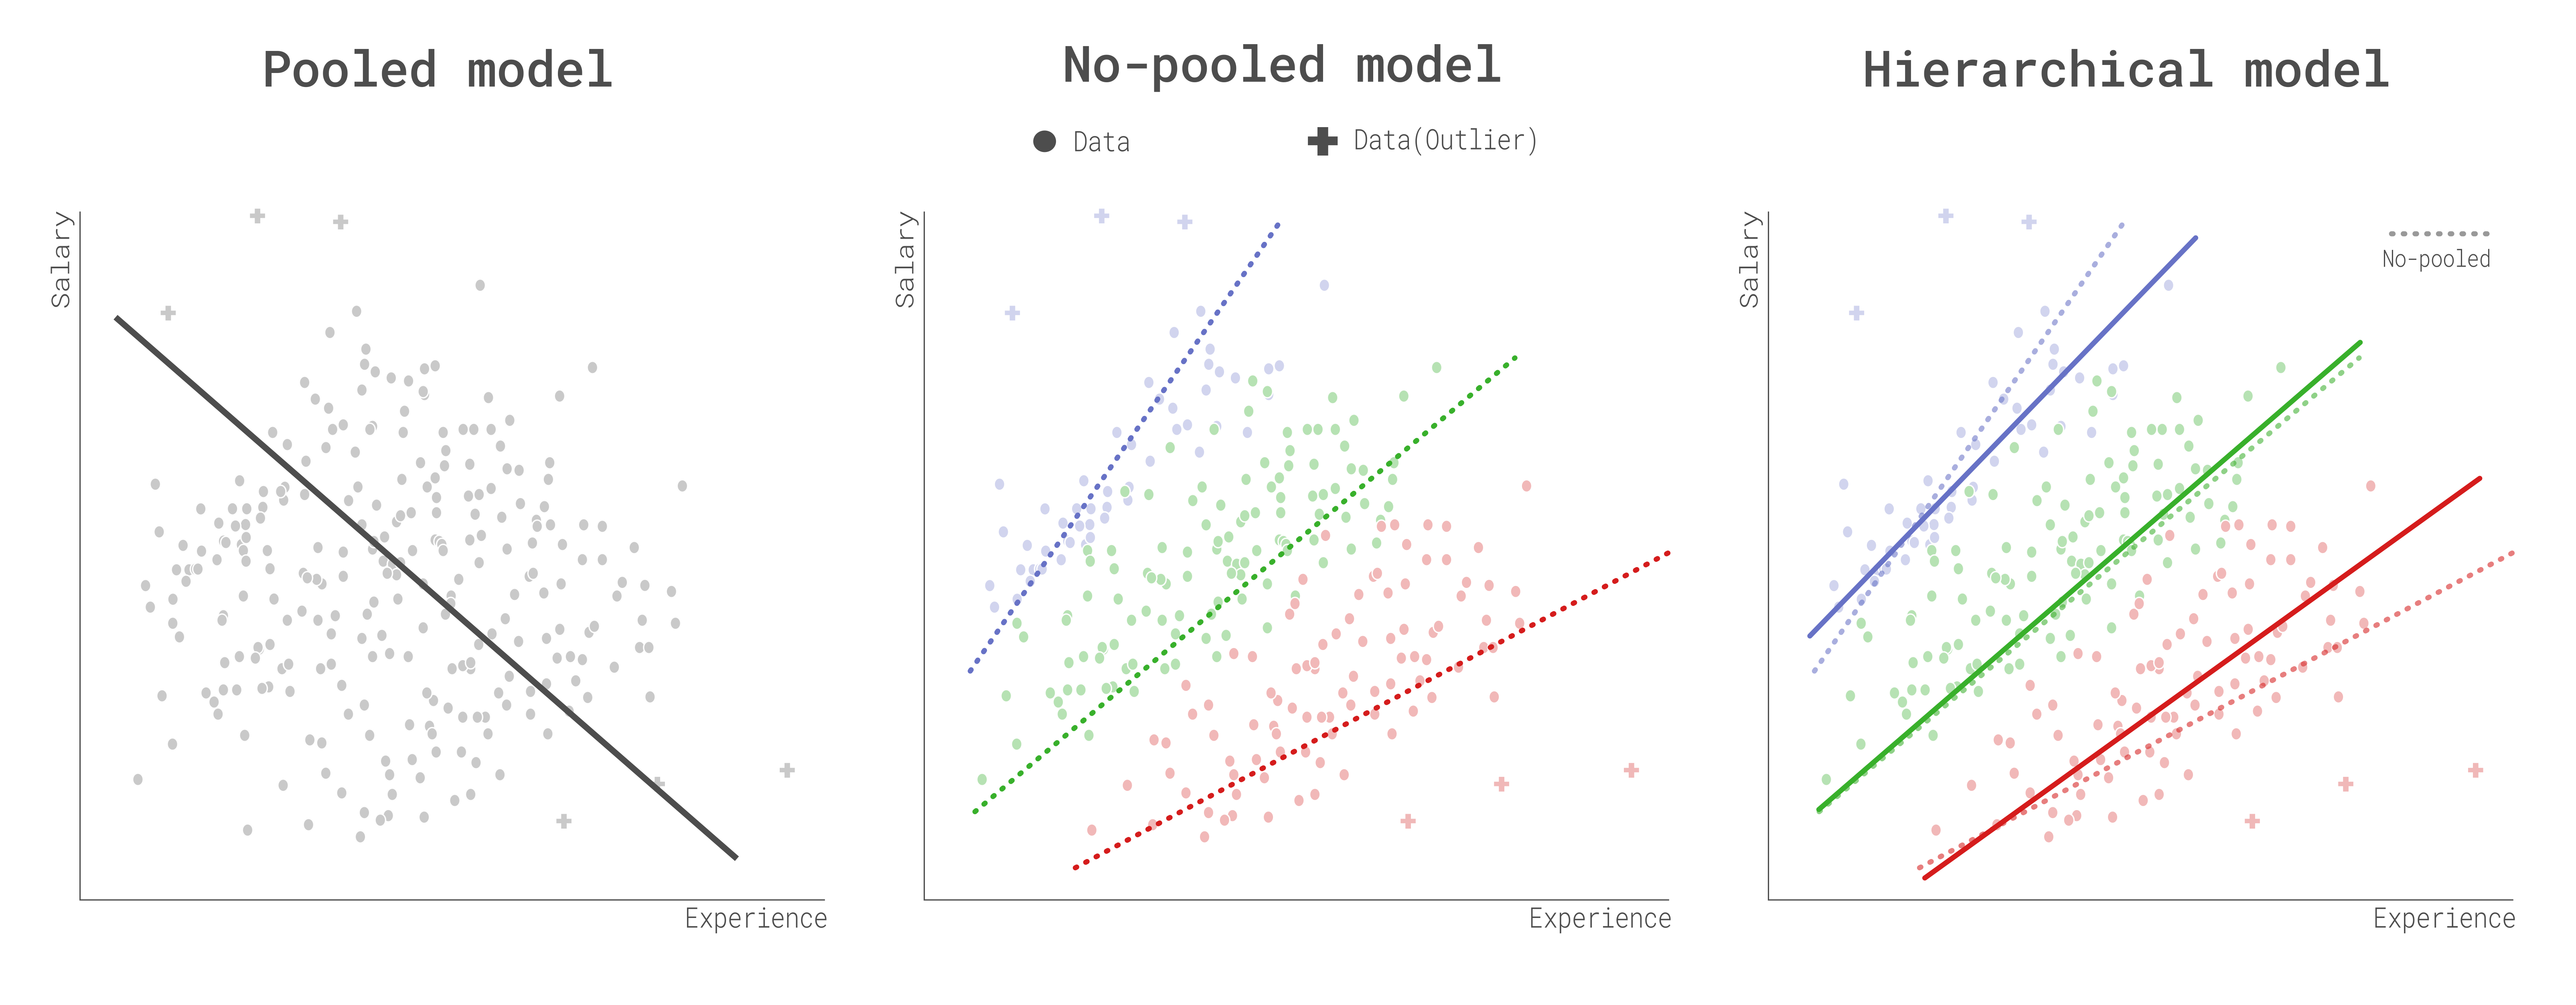
\includegraphics[width=1.0\textwidth]{images/ch5_simpsons_paradox/simpsons_paradox.png}
    \caption{Effect of model structure on the data representation}
    \label{fig:simpsons_paradox}
\end{figure}

Given that the hierarchical approach draws information from the higher level (industry level), salaries predicted for each category tend to move towards the average industry value, represented by the dashed lines in \Cref{fig:simpsons_paradox}. This behaviour is known as \textit{Shrinkage}, which can be interpreted as a regularization process that increases the model's robustness by reducing the effect of outliers and the risk of overfitting. 

As a brief overview, the following list and \Cref{fig:model_structure} summarize the differences in the inference process for the three approaches\footnote{There are similar model structures in the frequentist approach. The pooled and no-pooled counterpart could be a set of simple linear regressions or ANOVA models, and the Hierarchical model is known in the frequentist framework as a mixed-effects model. Numerous examples also exist in the random utility / discrete choice modelling literature.}

\begin{itemize}
    \item \textbf{Pooled model}: In this approach, the modeller defines a set of priors for each model parameter based on the existing knowledge. Then, the posterior distribution for each model parameter is estimated using the Bayesian framework reviewed in \Cref{chapter:bayesian_inference}. The posterior distributions represent the average value of each parameter for all industries and occupations. 

    \item \textbf{No-pooled model}: In this approach, each industry-occupation combination has a set of priors for each model parameter. Each prior is defined by the modeller based on the existent knowledge. Then, the estimation result is a distribution matrix for each model parameter. Each distribution in this matrix corresponds to the estimated posterior distribution for that specific industry occupation and that given parameter. 
    
    \item \textbf{Multilevel or Hierarchical model}: This approach follows the same process as the No-pooled model, adding an extra step before setting the priors. One of the key characteristics of the hierarchical models is the transfer of information between higher and lower levels. This is achieved by setting a set of hyperpriors that defines the localization and scale of the prior distributions (prior parameters). In the hierarchical approach, the modeller only defines the shape of the prior distribution and lets the data select the best parameters for that prior based on the hyperpriors. After the estimation process, a matrix of distributions for each model parameter is generated. Each one of these distributions corresponds to the estimated posterior distribution for that specific industry occupation and for that given parameter. However, each distribution shares information with other distributors in the same industry. The estimation process also provides posterior distributions for the hyperpriors, which corresponds to the distribution of the information shared across categories in the same industry. This process makes the hierarchical approach robust and powerful for modelling complex data structures.
\end{itemize}

\begin{figure}[H]
    \centering
    \includegraphics[width=0.78\textwidth]{images/ch5_model_structure/model_structure.png}
    \setlength{\abovecaptionskip}{-12pt}
    \caption{Inference process by model structure}
    \label{fig:model_structure}
\end{figure}

Despite these approaches exemplified in this section using linear models, it is important to highlight that these structures are model agnostic, which means that they can be used with linear and non-linear models. Therefore, the three approaches reviewed in this section only define the model structure. 

Based on these arguments, the Hierarchical structure seems to be the best option for modelling salaries using the SLID dataset. However, the model specification and selection sections compare the three approaches to measure their performance using the SLID data. In the model selection, the optimal model is chosen based on the measures reviewed in \Cref{section:goodness_of_fit}.

\section{Model variables}

The variables used in the model estimation are detailed in \Cref{table:model_vars}. It is important to highlight that all variables are used to select the model structure. After choosing the optimal structure, the final variables are selected through a Forward selection process, as presented in \Cref{section:model_selection}.

Based on the comments of \citet{Harmon2013}, the underestimation of the existent wage model could be related to the quality of the hourly salary data. Therefore, the proposed model uses annual salary as the target variable instead of the hourly wage. 

The original SLID dataset is split into two: from 1996 to 2007 and 2008 to 2011. The first corresponds to the dataset used in the model estimation, and the last is the dataset used in the validation section. 

\renewcommand{\arraystretch}{1.5}
\begin{table}[H]
    \begin{tabular}{p{2cm}p{4cm}p{2cm}p{7cm}}
        \textbf{Name} & \textbf{Units} & \textbf{Type} & \textbf{Description} \\
        \hline
        \rowcolor{lightgray} Experience & years & Continuous & Years of previous experience in the occupation and industry \\

        Sex & 0 or 1 & Categorical & Dummy variable that takes 0 for Males or 1 for Females \\

        \rowcolor{lightgray} Education Level & 0 or 1 for each education level: \newline No education, \newline Elementary, \newline High-school, \newline Postsecondary, \newline Undergraduate, \newline Graduate & Categorical & The dummy variable represents the education level using a One-hot encoding. \\

        Age & years (15-99) & Continuous & Age of the individual at the time of the survey \\

        \rowcolor{lightgray} Tenure & months & Continuous & Number of months in the same job \\

        Union & 0 or 1 & Categorical & Dummy variable that takes 1 if the individual is unionized or 0 otherwise \\

        \rowcolor{lightgray} Public sector & 0 or 1 & Categorical & The dummy variable takes 1 if the individual works in the public sector and 0 otherwise. \\

        Self-employment & 0 or 1 & Categorical & The dummy variable takes 1 if the individual is self-employed and 0 otherwise. \\

        \hline
    \end{tabular}
    \caption{\label{table:model_vars} Variables used in the model specification}
\end{table}


\section{Model specification}

Once the model structure and data variables are defined, it is necessary to specify the relationships between the variables of interest in the model by recreating the data generation process. Two of the most relevant characteristics of the data generation process are the distribution of the target variable and the relationships between the explanatory variables. 

As discussed in the exploratory data analysis section, salaries are positive and right-skewed distributed, which resembles the Gamma distribution. On the other hand, theoretical models explored in the literature review section show how the salary of a particular worker can be explained by using a linear combination of different personal attributes such as education level, experience, gender, and age, among others. Hence, the model specification must meet these target distribution and linearity requirements. 

A model that meets these requirements is the \textit{Gamma Generalized Linear Model (Gamma GLM)}, which belongs to the family of linear models that represents a process in terms of a linear combination with error distribution different from the normal distribution, as in the ordinary linear regression \citep{Nielsen2010}.

Given a set of explanatory variables $X=[X_1,X_2,...,X_p]$ and a set of model parameters $\theta = [\theta_0,\theta_1,...,\theta_p]$, the Gamma GLM is defined by the following components:

\begin{itemize}
    \item \textbf{Random component}: The response variable $Y$ follows a Gamma distribution (\Cref{eq:gamma_distribution}) defined by the parameters $\alpha$ and $\beta$ (shape and scale respectively). The expected value of this distribution is $\mu=\frac{\alpha}{\beta}$
    \begin{equation}\label{eq:gamma_distribution}
        f(y,\alpha, \beta)=\frac{\beta^\alpha}{\varGamma(\alpha)}y^{\alpha-1}e^{-\beta y} \text{ \\ \\ \\  , \\  \\ } y > 0
    \end{equation}
    \item \textbf{Systematic component}: The linear combination $\eta$ of explanatory variables $X$ and the model parameters $\theta$.
    \begin{equation}
        \eta = \theta_0 + \theta_1X_1+\theta_2X_2+...+\theta_pX_p
    \end{equation}
    \item \textbf{Link function}: This function connects the expected value of the target variable with the linear predictor $\eta$ using a log link and ensures that the linear predictor is positive and continuous. When solved for $\mu$, it provides the expectation over the target variable.
    \begin{align}
        \begin{split}
            log(\mu) &= \eta\\
            \mu &= e^{\eta}=e^{\theta_0+\theta_1X_1+...+\theta_pX_p}
        \end{split}
    \end{align}
\end{itemize}

Hence, the inference process is focused on estimating the parameters $\theta$'s in the systematic component, whereas the parameters $\alpha$ and $\beta$ in the random component are inferred indirectly using the systematic component and the log-link function. The following subsections present the model specification of the Gamma GLM for each model structure (Pooled, No-Pooled, and Hierarchical). 

\subsection{Pooled model}

\Cref{eq:pooled_model} presents the model specification for the Pooled structure and \Cref{fig:model_graph_pooled}. Model graph - Pooled shows the model graph. The expression \Cref{eq:pooled_model}-[1] corresponds to the random component, while the expressions \Cref{eq:pooled_model}-[2] and \Cref{eq:pooled_model}-[4] correspond to the priors for the model parameters $\theta_p$ and $\alpha$. The model parameters correspond to all variables listed in \Cref{table:model_vars}.

\begin{gather}
    \begin{split}
        Y \sim Gamma(\alpha,\beta) \quad \textcolor{gray}{[\text{1}]} \\
        \alpha \sim Uniform(0, 100) \quad \textcolor{gray}{[\text{2}]} \\
        \beta=\alpha/\mu \quad \textcolor{gray}{[\text{3}]} \\
        \theta_{p} \sim Normal(0, 1) \quad \textcolor{gray}{[\text{4}]} \\
        \mu=e^{\theta_0+\theta_{1}X_{1}+...+\theta_{p}X_{p}} \quad \textcolor{gray}{[\text{5}]} \\
    \end{split}
    \label{eq:pooled_model}
\end{gather}

The choice of the priors is given by: 
\begin{itemize}
    \item For the parameters $\theta$'s, the prior selected is the normal distribution with mean 0 and sigma 1. The mean centred in 0 ensures that the parameters can take positive or negative values according to the relationships in the data. 

    \item For the parameter $\alpha$, the prior selected is the uniform distribution with lower limit 0 and upper limit 100. The uniform distribution is a non-informative prior that ensures different values for $\alpha$ are tested with equal probability of occurrence. This choice is made because there is no evidence of the $\alpha$ value in previous salary prediction exercises. 
    
    \item The parameter $\beta$ does not require a prior because it is calculated based on the other parameters. 
\end{itemize}

\begin{figure}[H]
    \centering
    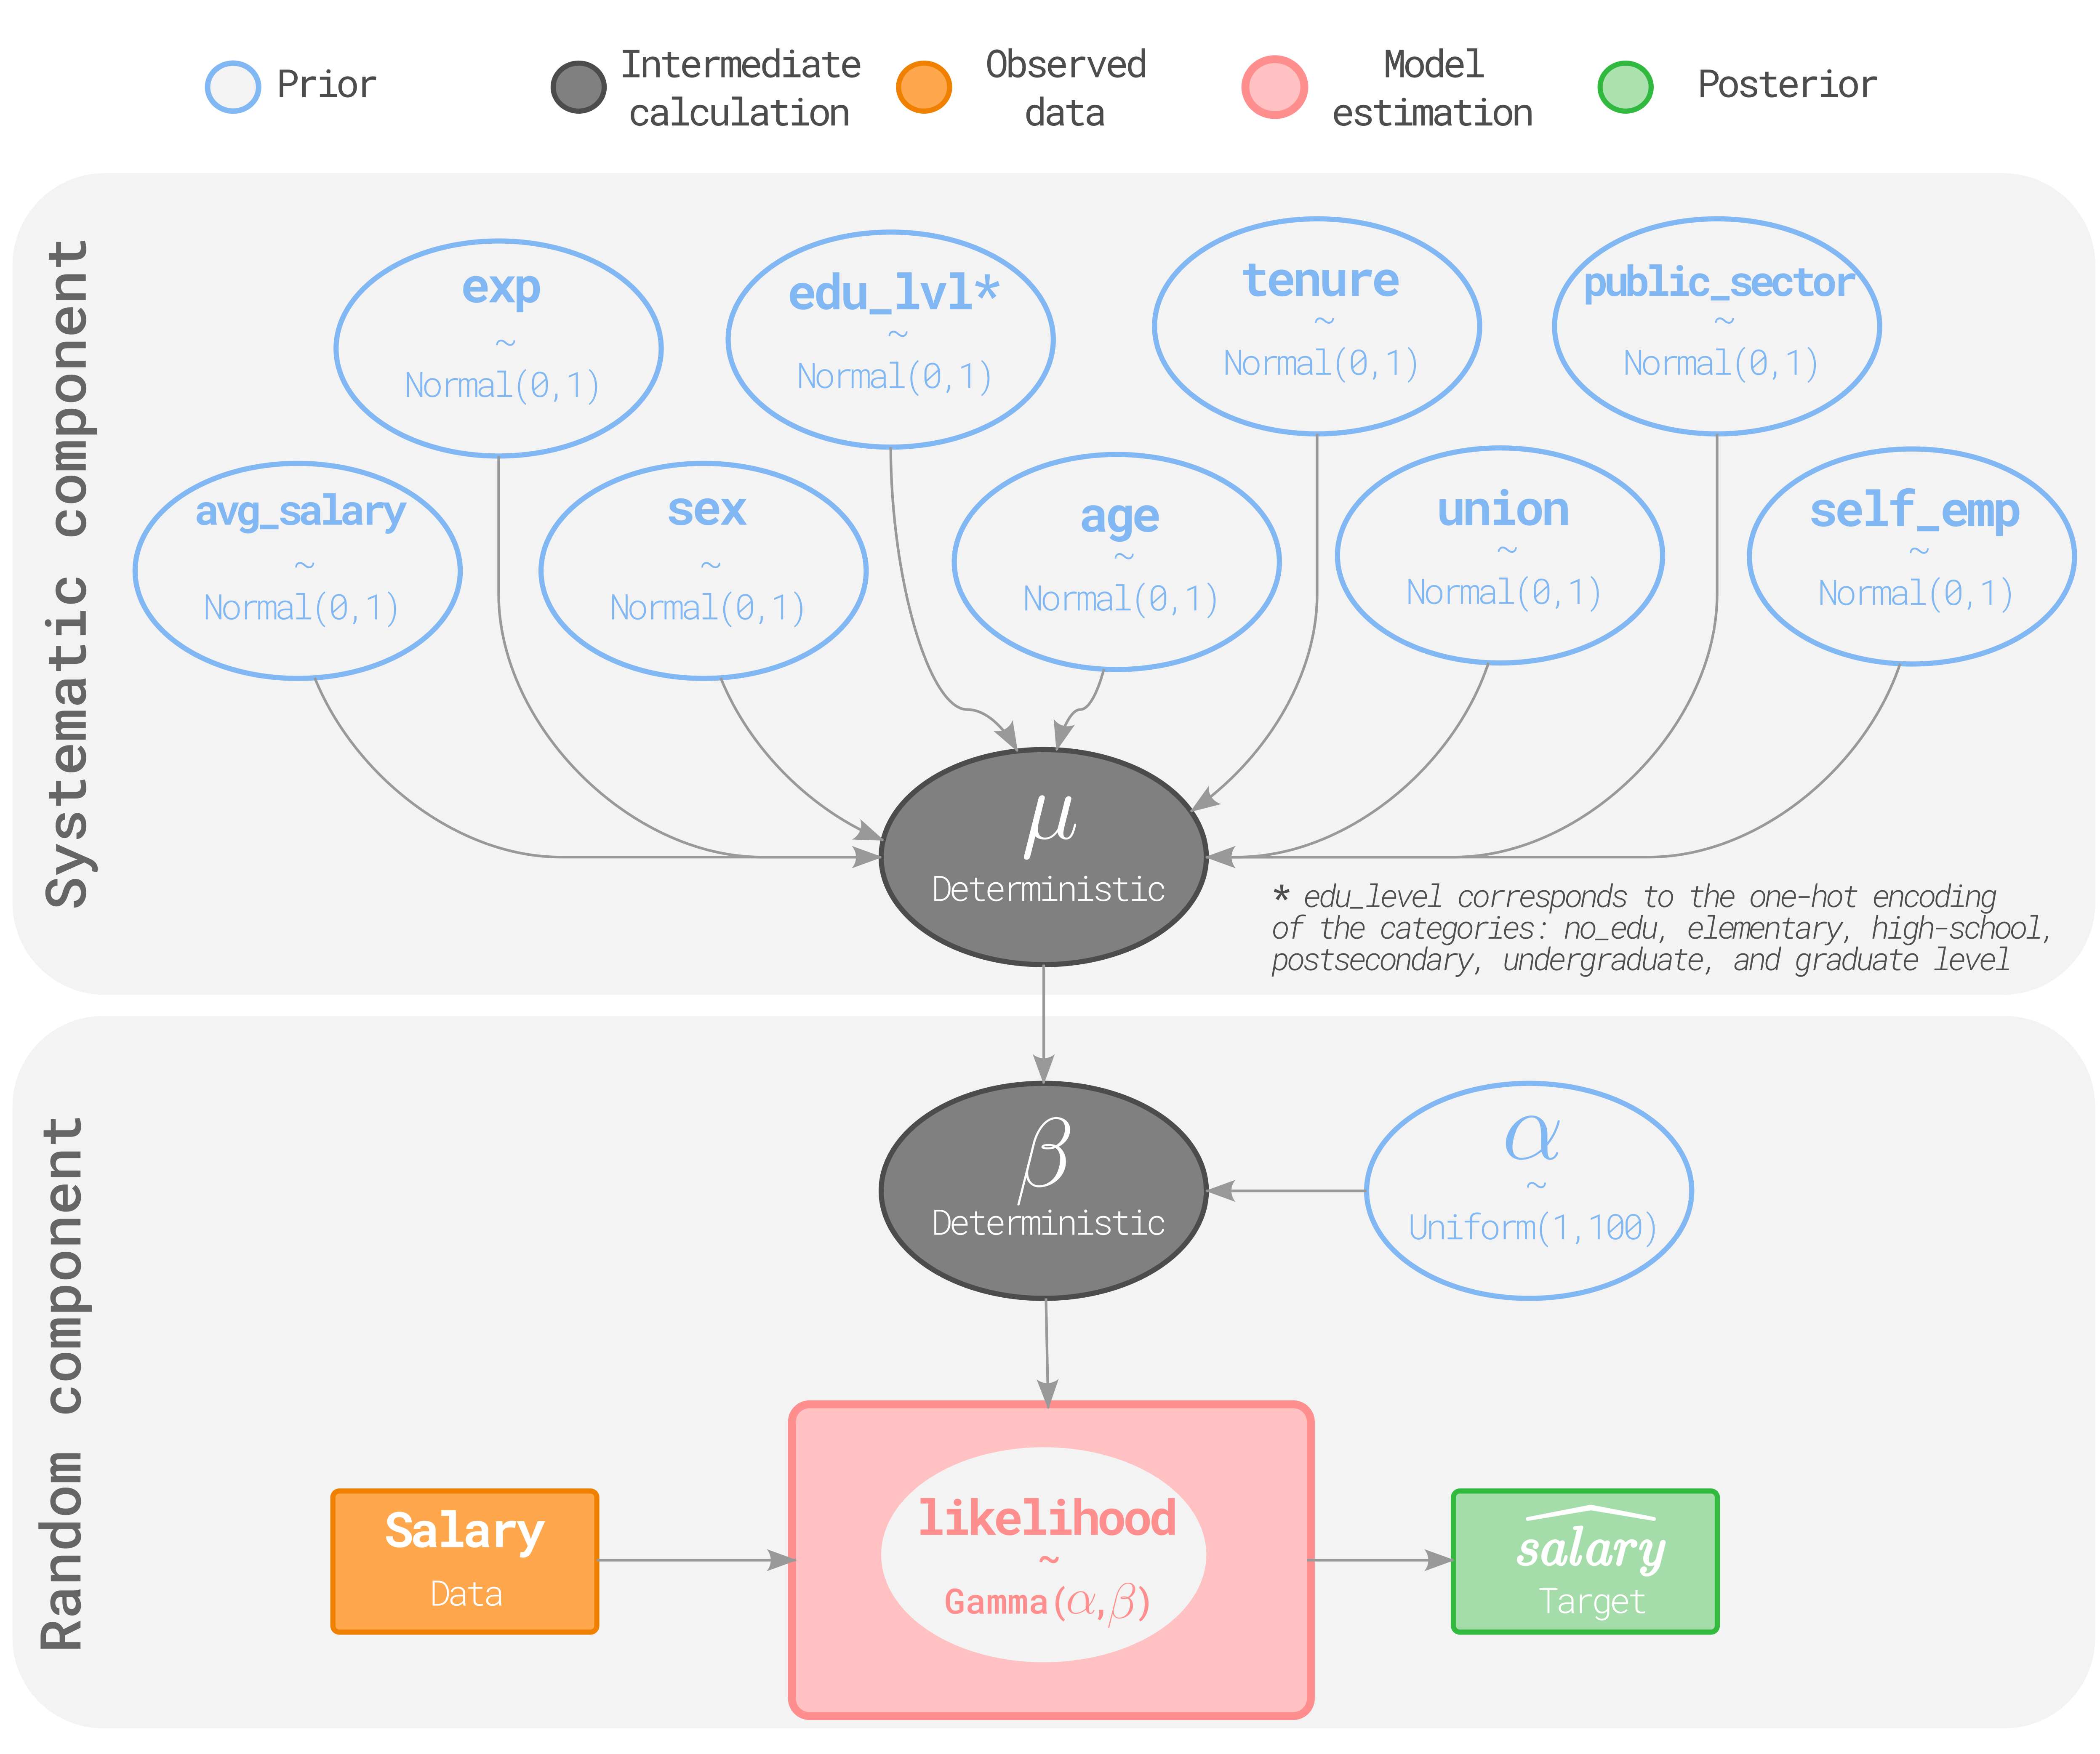
\includegraphics[width=0.96\textwidth]{images/ch5_pooled_graph/pooled_graph.png}
    \setlength{\abovecaptionskip}{-12pt}
    \caption{Model graph - Pooled}
    \label{fig:model_graph_pooled}
\end{figure}

\subsection{No-pooled model} 

\Cref{eq:no_pooled_model} presents the model specification for the No-pooled structure, and \Cref{fig:model_graph_nopooled} shows the model graph. The model parameters correspond to all variables listed in \Cref{table:model_vars}. The superscripts $ind$  and $occ$ correspond to each hierarchy level (industries and occupations) presented in \Cref{section:hierarchy}. 

\begin{gather}
    \begin{split}
        Y \sim Gamma(\alpha,\beta) \quad \textcolor{gray}{[\text{1}]} \\
        \alpha \sim Uniform(0, 100) \quad \textcolor{gray}{[\text{2}]} \\
        \beta=\alpha/\mu \quad \textcolor{gray}{[\text{3}]} \\
        \theta_{p}^{ind} \sim Normal(0, 1) \quad \textcolor{gray}{[\text{4}]} \\
        \theta_{p}^{occ} \sim Normal(0, 1) \quad \textcolor{gray}{[\text{5}]} \\
        \eta^{ind} = \theta_0^{ind}+\theta_1^{ind}X_1+...+\theta_p^{ind}X_p \quad \textcolor{gray}{[\text{6}]} \\
        \eta^{occ} = \theta_0^{occ}+\theta_1^{occ}X_1+...+\theta_p^{occ}X_p \quad \textcolor{gray}{[\text{7}]} \\
        \mu=e^{\eta^{ind}+\eta^{occ}} \quad \textcolor{gray}{[\text{8}]} \\
    \end{split}\label{eq:no_pooled_model}
\end{gather}

Like in the Pooled model, the choice of the priors in the No-pooled model is given by: 
\begin{itemize}
    \item For the parameters $\theta$'s for both $ind$ and $occ$, the prior selected is the normal distribution with mean 0 and sigma 1. 

    \item For the parameter $\alpha$, the prior selected is the uniform distribution with lower limit 0 and upper limit 100. 
    
    \item The parameter $\beta$ does not require a prior because it is calculated based on the other parameters. 
\end{itemize}

\begin{figure}[H]
    \centering
    \includegraphics[width=0.96\textwidth]{images/ch5_no_pooled_graph/no_pooled_graph.png}
    \setlength{\abovecaptionskip}{-12pt}
    \caption{Model graph - No-pooled}
    \label{fig:model_graph_nopooled}
\end{figure}

\subsection{Hierarchical model}

\Cref{eq:hierarchical_model} presents the model specification for the Hierarchical model, and \Cref{fig:model_graph_hierarchical} shows the model graph. The hierarchical model uses the variables listed in \Cref{table:model_vars} and superscripts $ind$  and $occ$ presented in \Cref{section:hierarchy}. However, it adds two hyperpriors (one for the localization parameter and one for the scale parameter) that share information from a higher to a lower level. These hyperpriors are defined for both the industry and occupation level.  

 \begin{gather}
    \begin{split}
        Y \sim Gamma(\alpha,\beta) \quad \textcolor{gray}{[\text{1}]} \\
        \alpha \sim Uniform(0, 100) \quad \textcolor{gray}{[\text{2}]} \\
        \beta=\alpha/\mu \quad \textcolor{gray}{[\text{3}]} \\
        loc_{p}^{ind} \sim Normal(0,1) \quad \textcolor{gray}{[\text{4}]} \\
        scale_{p}^{ind} \sim HalfNormal(1) \quad \textcolor{gray}{[\text{5}]} \\
        loc_{p}^{occ} \sim Normal(0,1) \quad \textcolor{gray}{[\text{6}]} \\
        scale_{p}^{occ} \sim HalfNormal(1) \quad \textcolor{gray}{[\text{7}]} \\
        \theta_{p}^{ind} \sim Normal(loc_{p}^{ind}, scale_{p}^{ind}) \quad \textcolor{gray}{[\text{8}]} \\
        \theta_{p}^{occ} \sim Normal(loc_{p}^{occ}, scale_{p}^{occ}) \quad \textcolor{gray}{[\text{9}]} \\
        \eta^{ind} = \theta_0^{ind}+\theta_1^{ind}X_1+...+\theta_p^{ind}X_p \quad \textcolor{gray}{[\text{10}]} \\
        \eta^{occ} = \theta_0^{occ}+\theta_1^{occ}X_1+...+\theta_p^{occ}X_p \quad \textcolor{gray}{[\text{11}]} \\
        \mu=e^{\eta^{ind}+\eta^{occ}} \quad \textcolor{gray}{[\text{12}]} \\
    \end{split}\label{eq:hierarchical_model}
 \end{gather}

 The choice of the priors in the Hierarchical model is given by: 
\begin{itemize}
    \item For the hyperprior $loc_p^*$, the distribution selected is the Normal distribution with mean 0 and sigma 1. That allows the model to choose the best value according to the observed data and share the same distribution for occupations in the same industry. 

    \item Likewise, the hyperprior $scale_p^*$ is defined with the Half-Normal distribution with sigma 1. This distribution ensures that all values are positive, which is mandatory given that $scale_p^*$ is the sigma value in the correspondent prior $\theta_p^*$. 

    \item For the parameters $\theta$'s for both $ind$ and $occ$, the prior selected is the normal distribution with mean $loc_p^*$ and sigma $scale_p^*$. 

    \item For the parameter $\alpha$, the prior selected is the uniform distribution with lower limit 0 and upper limit 100. 

    \item The parameter $\beta$ does not require a prior because it is calculated value. 
\end{itemize}

\begin{figure}[H]
    \centering
    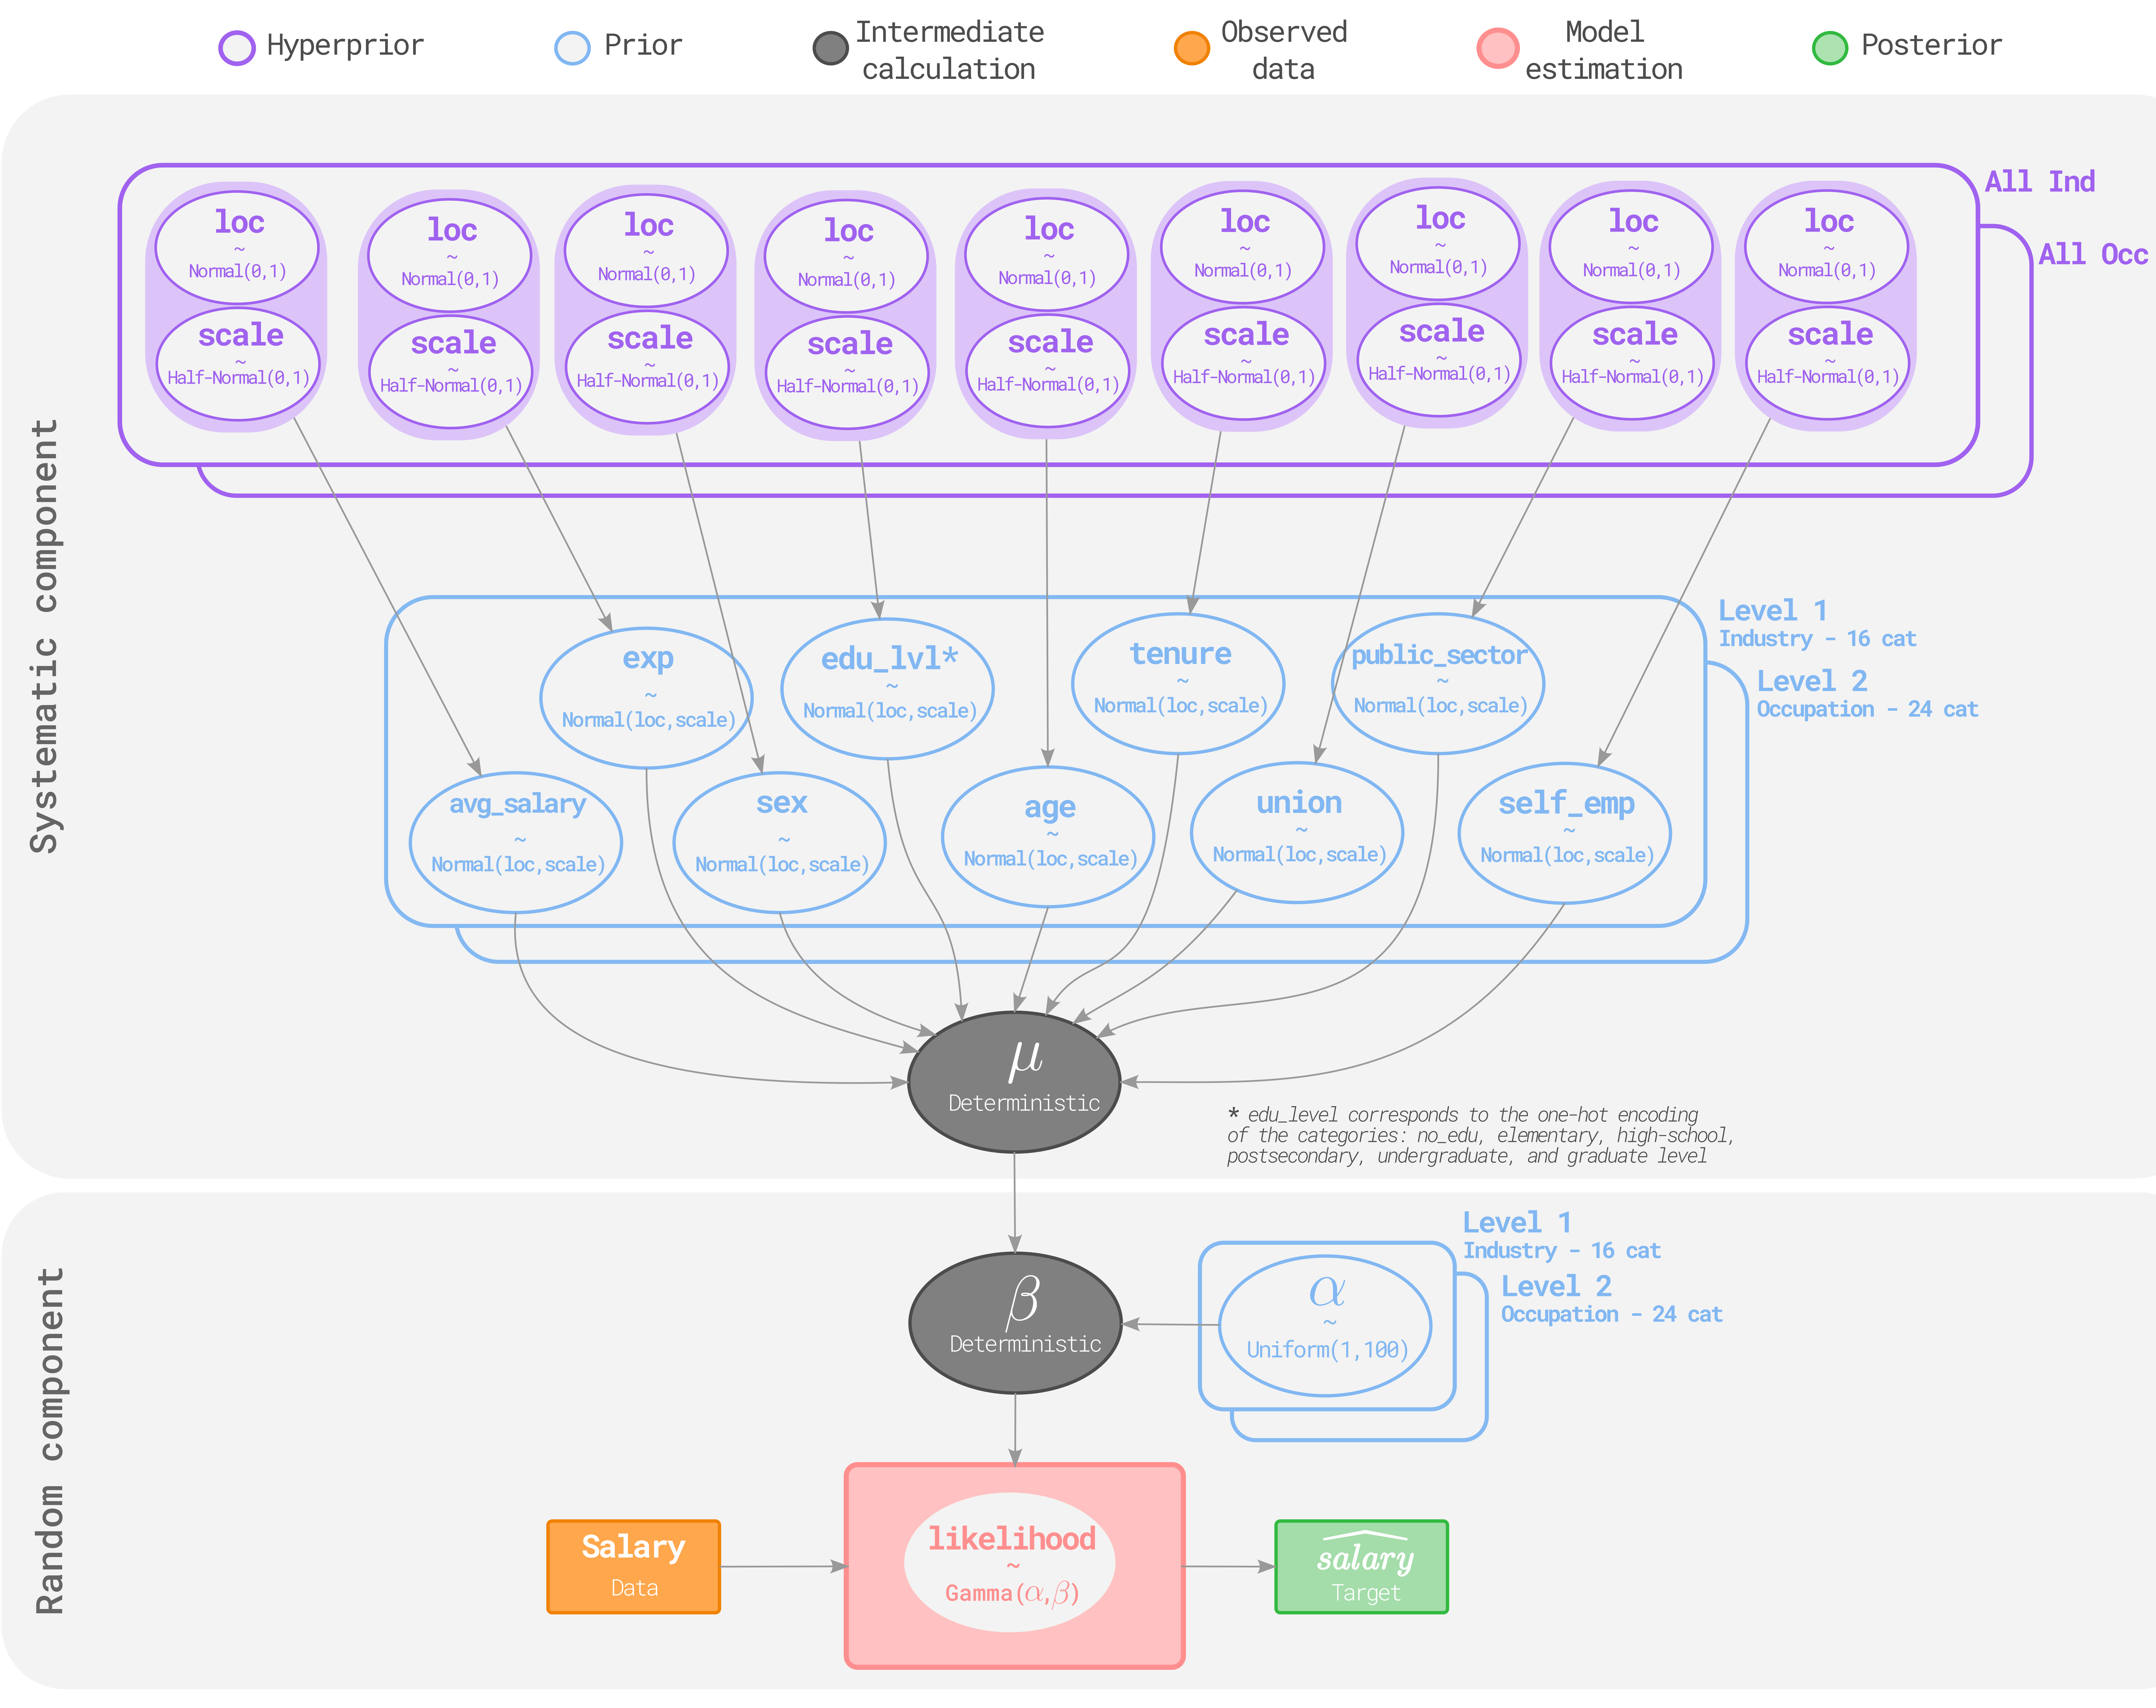
\includegraphics[width=0.96\textwidth]{images/ch5_hierarchical_graph/hierarchical_graph.png}
    \setlength{\abovecaptionskip}{-12pt}
    \caption{Model graph - Hierarchical}
    \label{fig:model_graph_hierarchical}
\end{figure}

\section{Model selection}\label{section:model_selection}

After running the inference on the three model structures, the results are compared using the performance metrics presented in \Cref{section:goodness_of_fit}. The model selection is divided into two sequential parts: 1) the model structure selection, which selects the best performing model between the pooled, no-pooled, and hierarchical structure, and 2) based on the structure selection, this part focuses on the most relevant variables based on model performance. The result from the 2-stage selection process is the optimal model, which is the proposal to replace the existing wage model in the labour market module of the ILUTE framework. 

\subsection{Structure selection: Pooled vs. No-pooled vs. Hierarchical model}\label{section:structure_selection} 

\Cref{fig:model_comparison} shows a model comparison using the LOO-CV measure (ELPPD score) and the WAIC score. The maximization of the ELPPD minimizes the KL divergence. Hence, in this figure, the higher the elppd value, the better the model.

\begin{figure}[H]
    \centering
    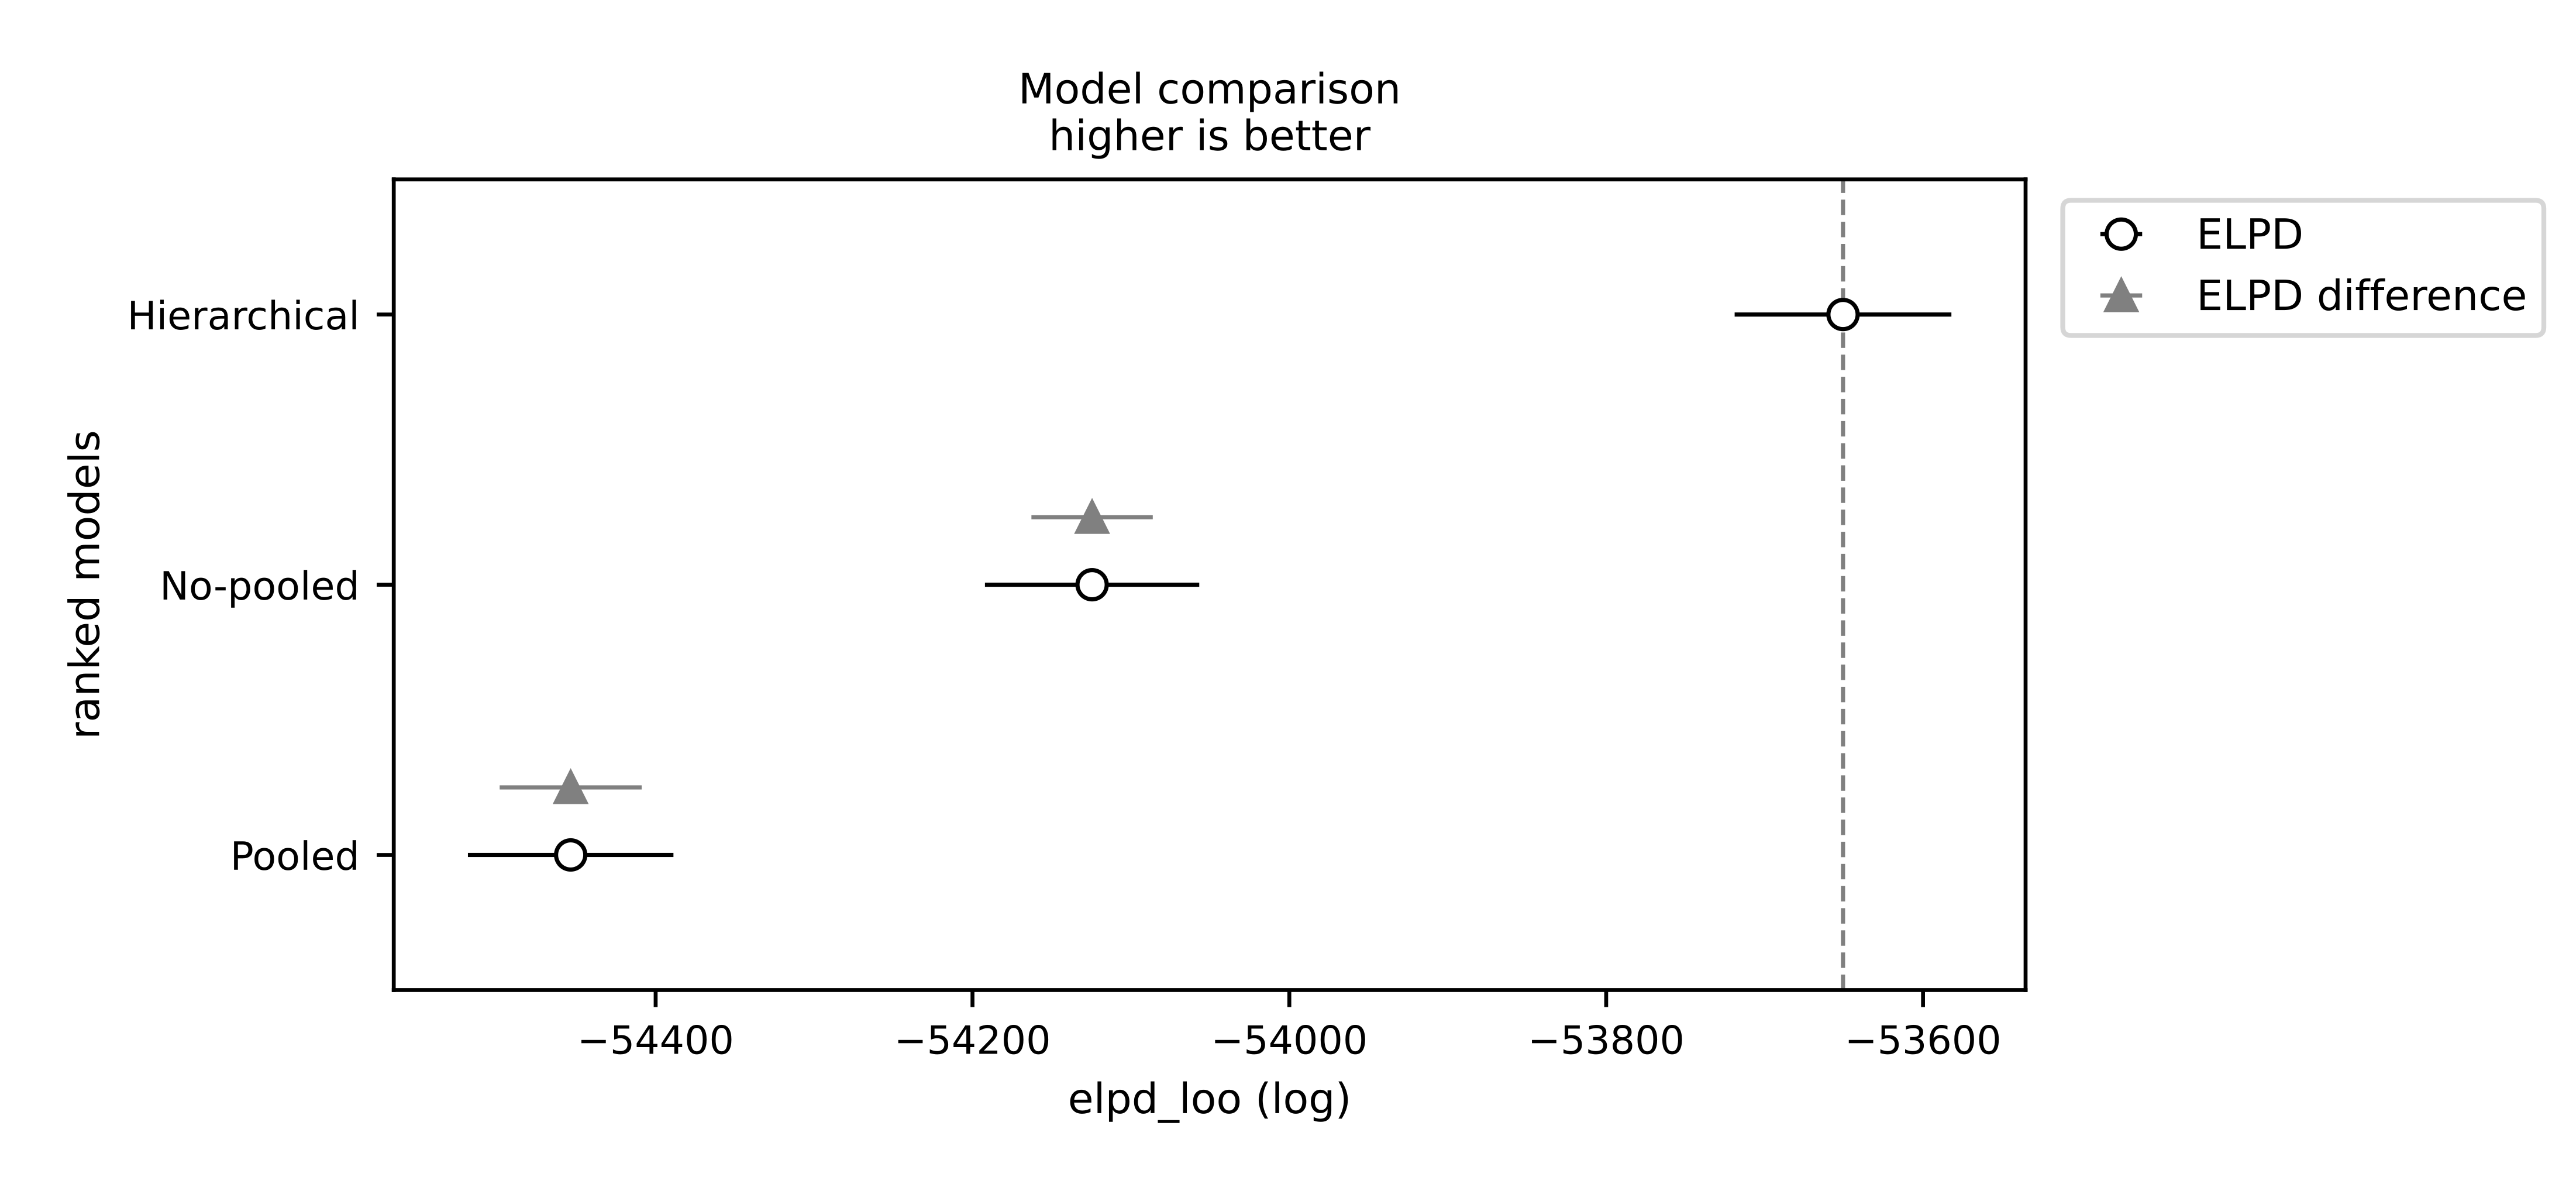
\includegraphics[width=0.96\textwidth]{images/ch5_model_structure_comparison/model_structure_comparison.png}
    \setlength{\abovecaptionskip}{-12pt}
    \caption{Model structure comparison }
    \label{fig:model_comparison}
\end{figure}

As expected, the hierarchical model shows better performance than the other approaches. The white circle represents the point estimate of the ELPPD-LOO score that measures the out-of-sample model performance. In contrast, the horizontal lines represent the uncertainty or error bars for the point estimate. Likewise, the ELPD difference provides a measure of comparison between each model and the reference model (best performant). The in-sample point estimate measures the model performance with the data used in the model estimation.  

The in-sample ELPPD score is an estimate of the performance of the training dataset. In contrast, the ELPPD-LOO score is an estimate of the performance on the validation dataset, which is a better estimate of the model performance in a real setting. The comparison between these two values ensures that the model is not overfitting. As expected, the model's performance in the in-sample case (training data) is higher than the out-of-sample case (validation data), which implies that the \textit{shrinkage effect} of the hierarchical approach is improving the performance by reducing the model complexity and avoiding overfitting. 

The results in \Cref{fig:model_comparison} confirm that the hierarchical structure provides a higher predictive power than the pooled and no-pooled approach. Including the hyperpriors allows the model to better capture the complex relationships and dependencies in the data compared to the other approaches (pooled and no-pooled). Therefore, from this point, all tests and additional runs are performed using the hierarchical structure.

\subsection{Forward variable selection} 

After selecting the optimal model structure, a Forward selection process is performed on the variables set to choose the most relevant from the predictive perspective. This process starts from the most straightforward model representation to the total variable set by adding one variable at each step. The simplest model corresponds to an intercept model (fixed effects), representing the average salary for that industry and that occupation. 

\Cref{fig:forward_selection} compares each variable addition from the simplest model to the one with the complete set of variables. These models are ranked from the best to the worst in terms of model performance, using the same ELPPD-LOO and WAIC scores used in the model structure selection.

\begin{figure}[H]
    \centering
    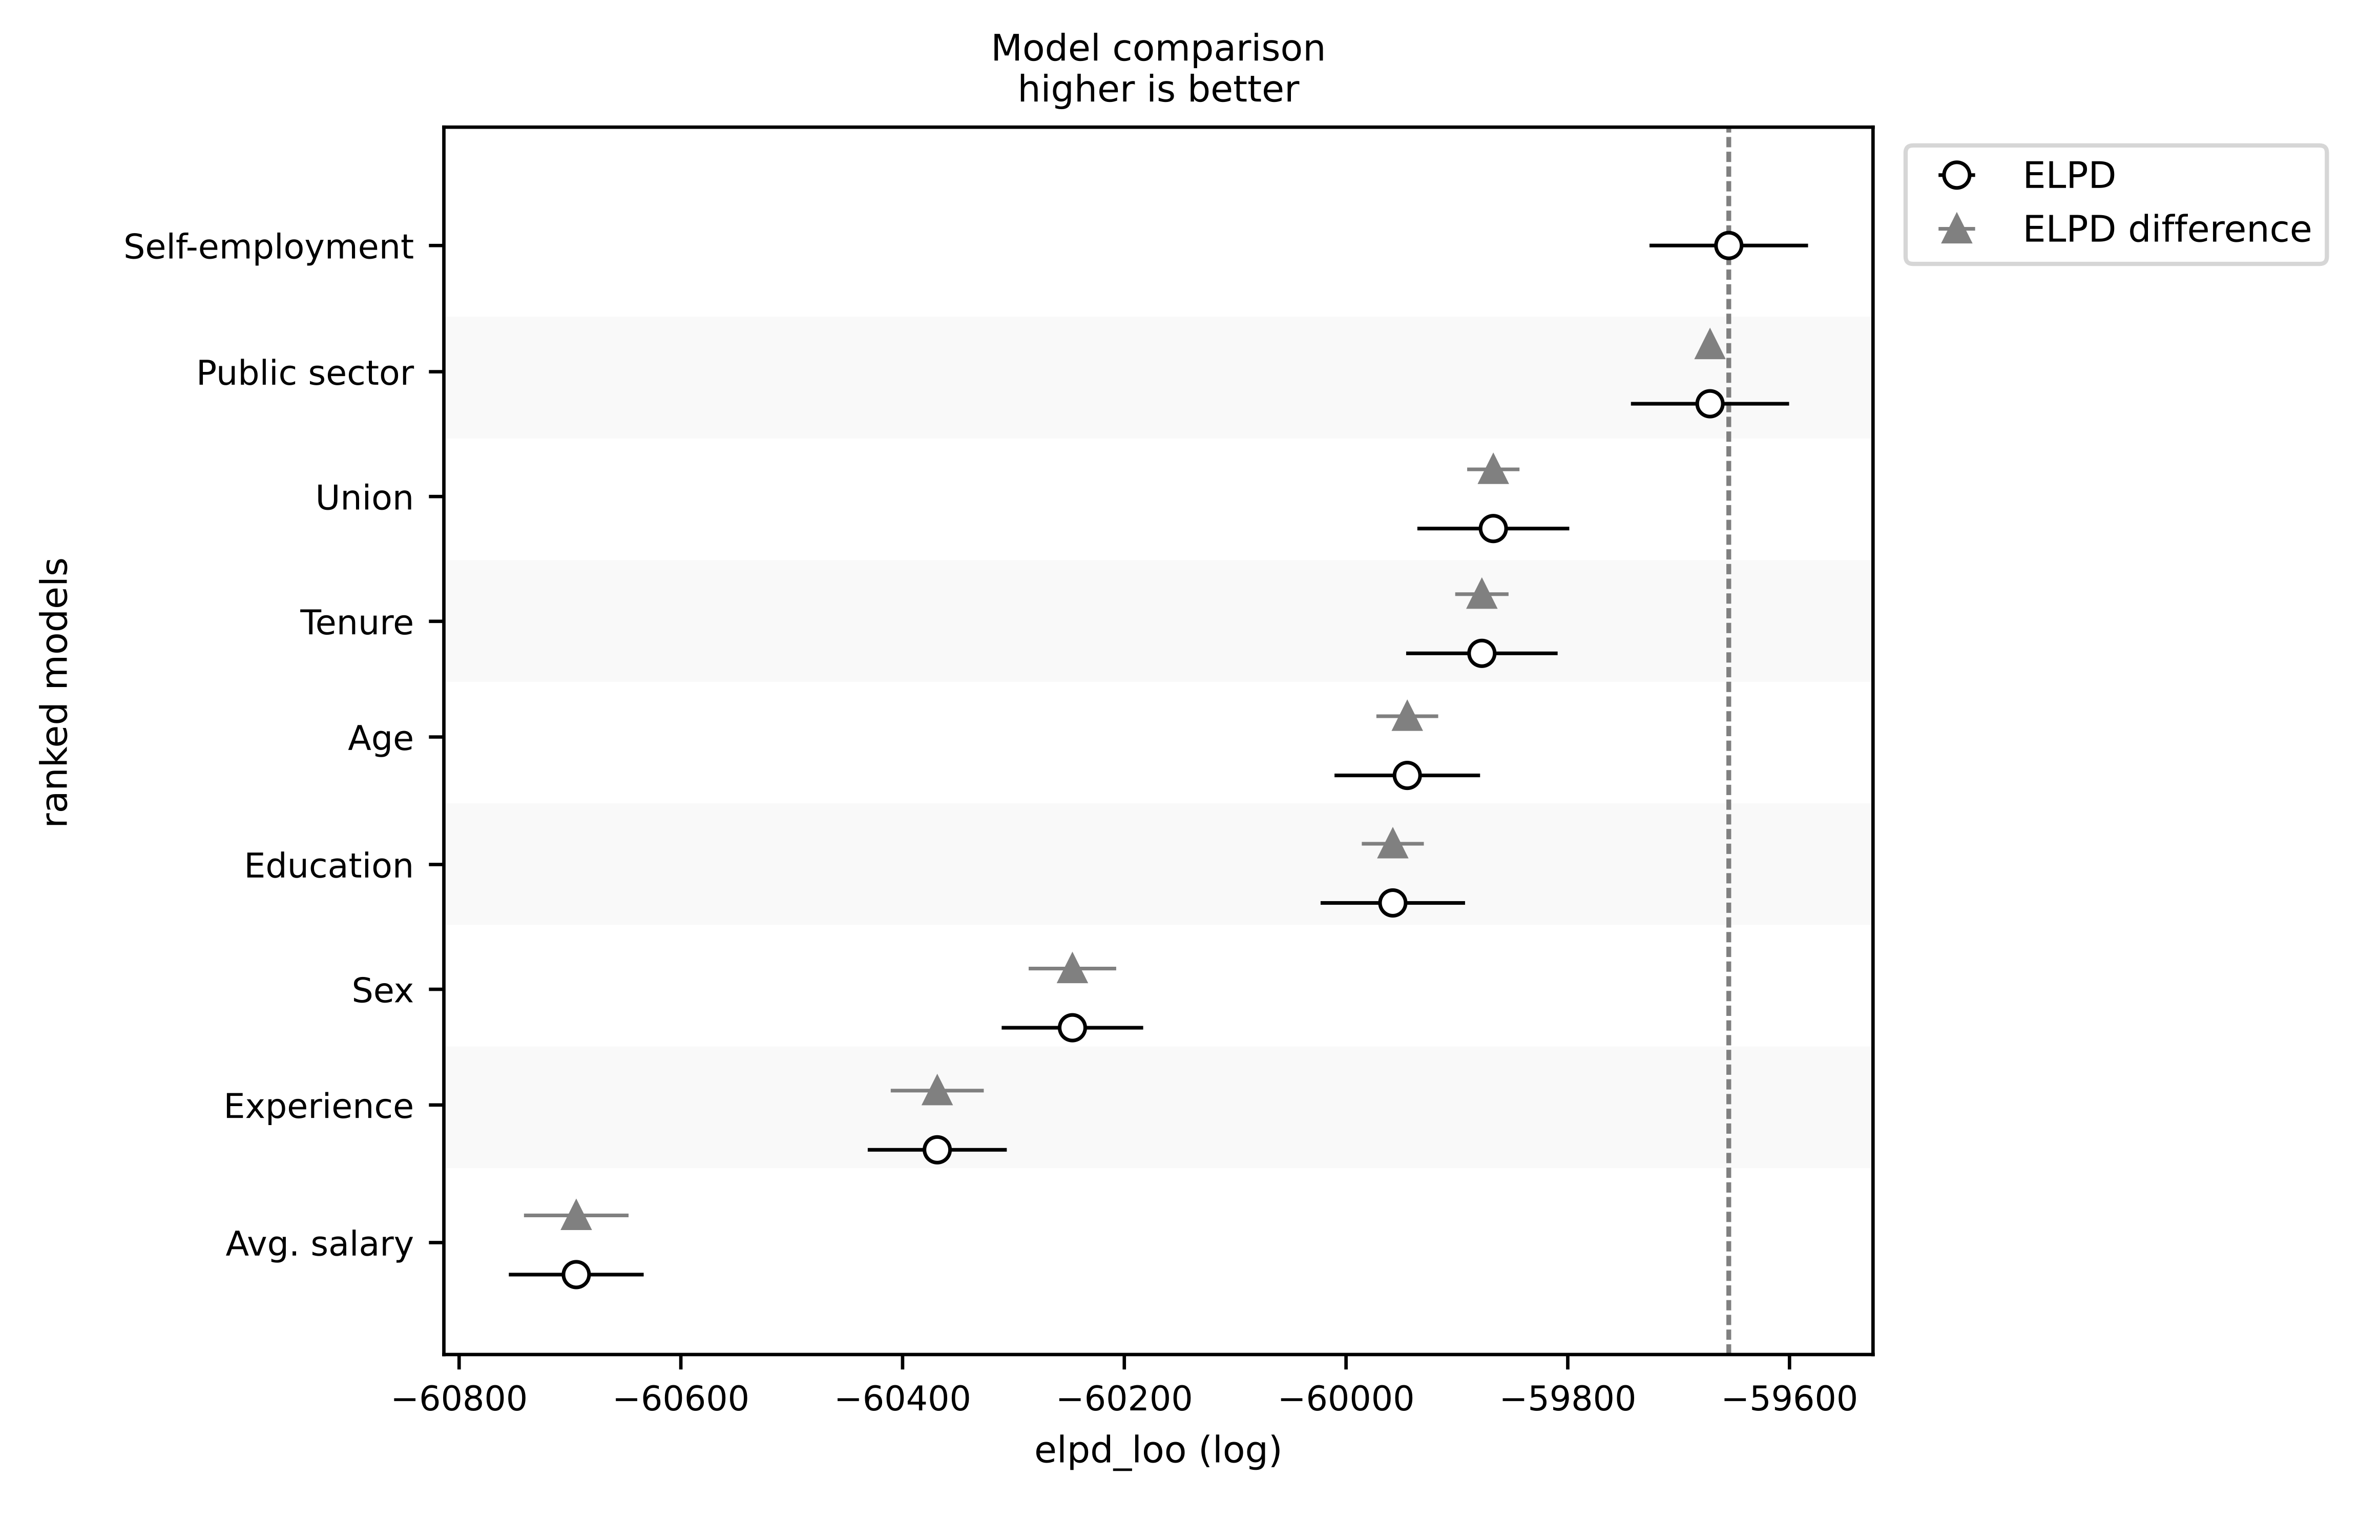
\includegraphics[width=0.8\textwidth]{images/ch5_forward_sel/forward_sel.png}
    \setlength{\abovecaptionskip}{-5pt}
    \caption{Forward variable selection}
    \label{fig:forward_selection}
\end{figure}

Starting from the intercept (avg\_salary), each variable is added to the model and the \textit{elpd} measure is calculated. Although adding each variable improves the model performance, the variables with the most significant effect on the target variable are experience, sex, education, and employment sector. These results are in line with the theoretical models and the literature review. On the other hand, variables such as age, tenure, and self-employment add little or no information at all, so they can be dropped from the model without losing significant performance. This selection process helps to reduce the model complexity and reduces the risk of overfitting the data.

Based on this variable selection process, the optimal model contains the predictors: \textbf{\textit{Avg\_salary, Experience, Sex, Education, Union and Public Sector}}. \Cref{fig:final_posterior} shows a subset of the posterior distributions for some industries and occupations in the final model. The chart with all model parameters is presented in \Cref{app:posterior_dists_final}.

\begin{figure}[H]
    \centering
    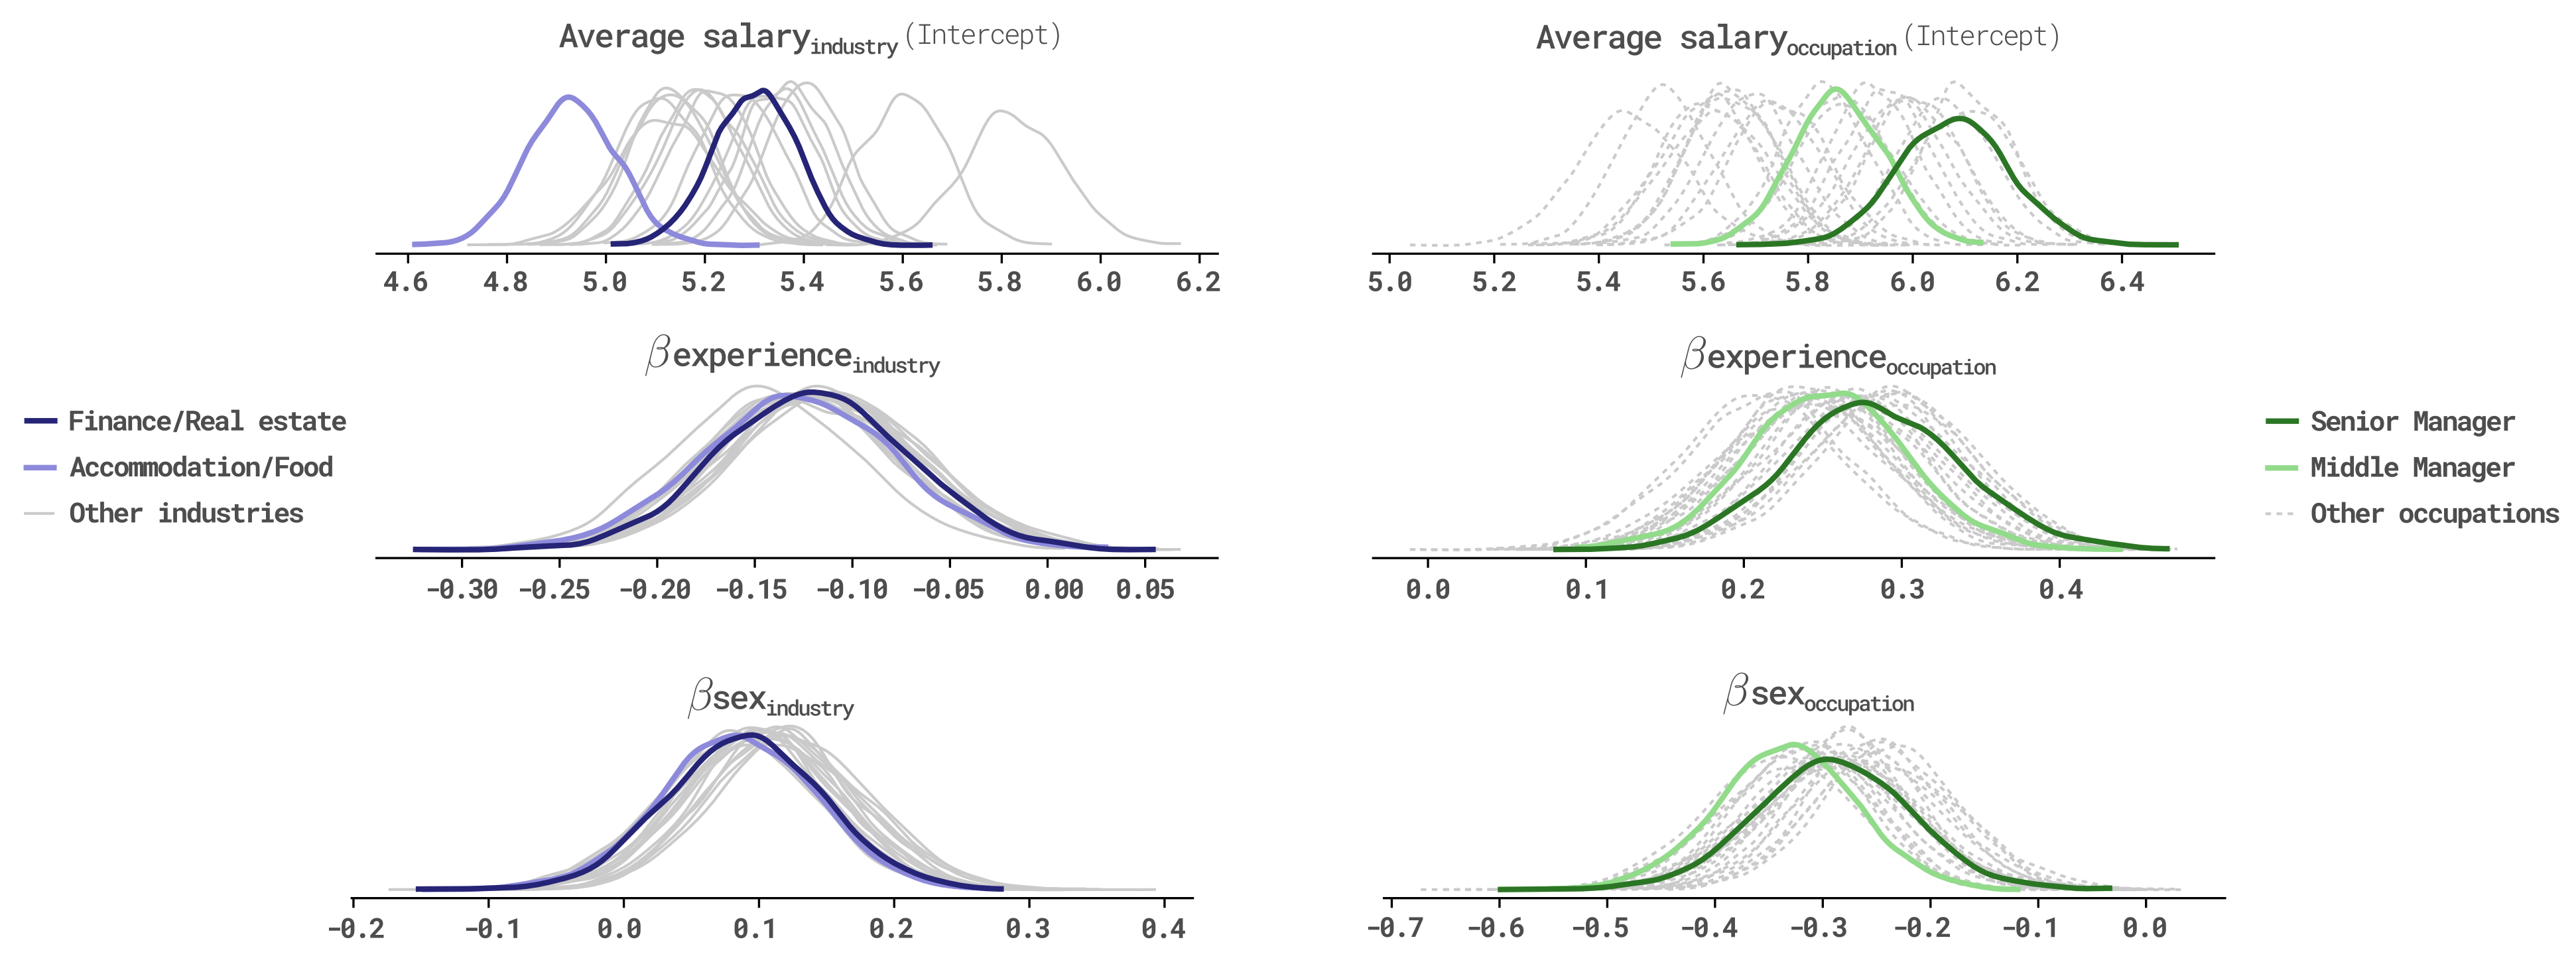
\includegraphics[width=1.0\textwidth]{images/ch5_traces/trace_1.png}
    \setlength{\abovecaptionskip}{-5pt}
    \caption{Posterior distributions for some industries and occupations in the final model}
    \label{fig:final_posterior}
\end{figure}

\section{Model interpretability}

The following bullets discuss the main results based on the posterior parameter distributions obtained from the Optimal model (after forward selection). It is important to highlight that although these results are in line with theory, they reflect the cultural and societal conditions from 1996 to 2007: 

\begin{itemize}
    \item Given that the Gamma GLM uses a log-link function, the relationship between the model parameters and the target variable is multiplicative\footnote{After applying the inverse of the log-link (exponential), which converts the value to the units of the data (CAD 2023)}. Therefore, the intercept (avg\_salary by industry and occupation) is interpreted as the base salary. Then, each parameter increases or reduces by a certain percentage of this salary base according to their effect (positive or negative)\footnote{After applying the inverse of the log-link (exponential)}. 

    \item As expected, most of the salary variability comes from the industry and occupation category, given the hierarchical structure of the labour market. In particular, the salaries of individuals in some physically demanding occupations (e.g. Construction trades) are explained mainly by their occupation rather than by the industry. This means this occupation has a low industry-base salary but higher occupation-base salaries than the other industries and occupations. 
    
    \item The gender gap is mainly explained by the negative values of the sex parameter related with occupation. Although this parameter is positive for industry level, when considering the overall effect (considering both industry and occupation value) the difference is negative for all industries and occupations. 
    
    \item Based on the forward selection results and the magnitude of the parameters, education level is the predictor that contributes the most to the variability explanation. As supported by the human capital theory, education is positively correlated with salaries across all industries and occupations. 
    
    \item Experience is a better predictor of salaries than job tenure because the latter is attached to the current job. Conversely, experience can be seen as a proxy for the skill set of an individual. Therefore, it provides more information about the potential salary of a candidate. 
    
    \item According to the model, public sector and union participation positively correlate with salaries. As public employees and unions can have more bargaining capacity, this could benefit the individuals in this sector and under union agreements. 
\end{itemize}

\section{Online learning: Longitudinal analysis of the estimated parameters }

Labour markets are constantly evolving. Some changes are observed in short periods, usually cyclical and related to the oscillation between supply and demand. In contrast, some changes are observed in more extended periods, usually related to technological, social, or political changes. The former is more straightforward to predict, while the latter is challenging because it usually corresponds to structural changes. Given the effect of the long-term changes in the labour market structure, the evolution of the model parameters through time becomes relevant for measuring the model validity and robustness to structural changes. 

The model performance can be assessed through time by comparing the estimated parameters using the whole dataset versus the estimated parameters using a sequential approach. This sequential estimation is aligned with the Bayesian inference framework because the posterior belief on the current period can become the prior belief for the next period. This approach is called \textit{Online learning}. 

Using the hierarchical model after the variable selection, \Cref{fig:online_learning_salary} to \Cref{fig:online_learning_sex} compare the evolution of the posterior distribution for some model parameters using Online Learning and the same parameter posterior distributions estimated with the whole dataset. 

\begin{figure}[H]
    \centering
    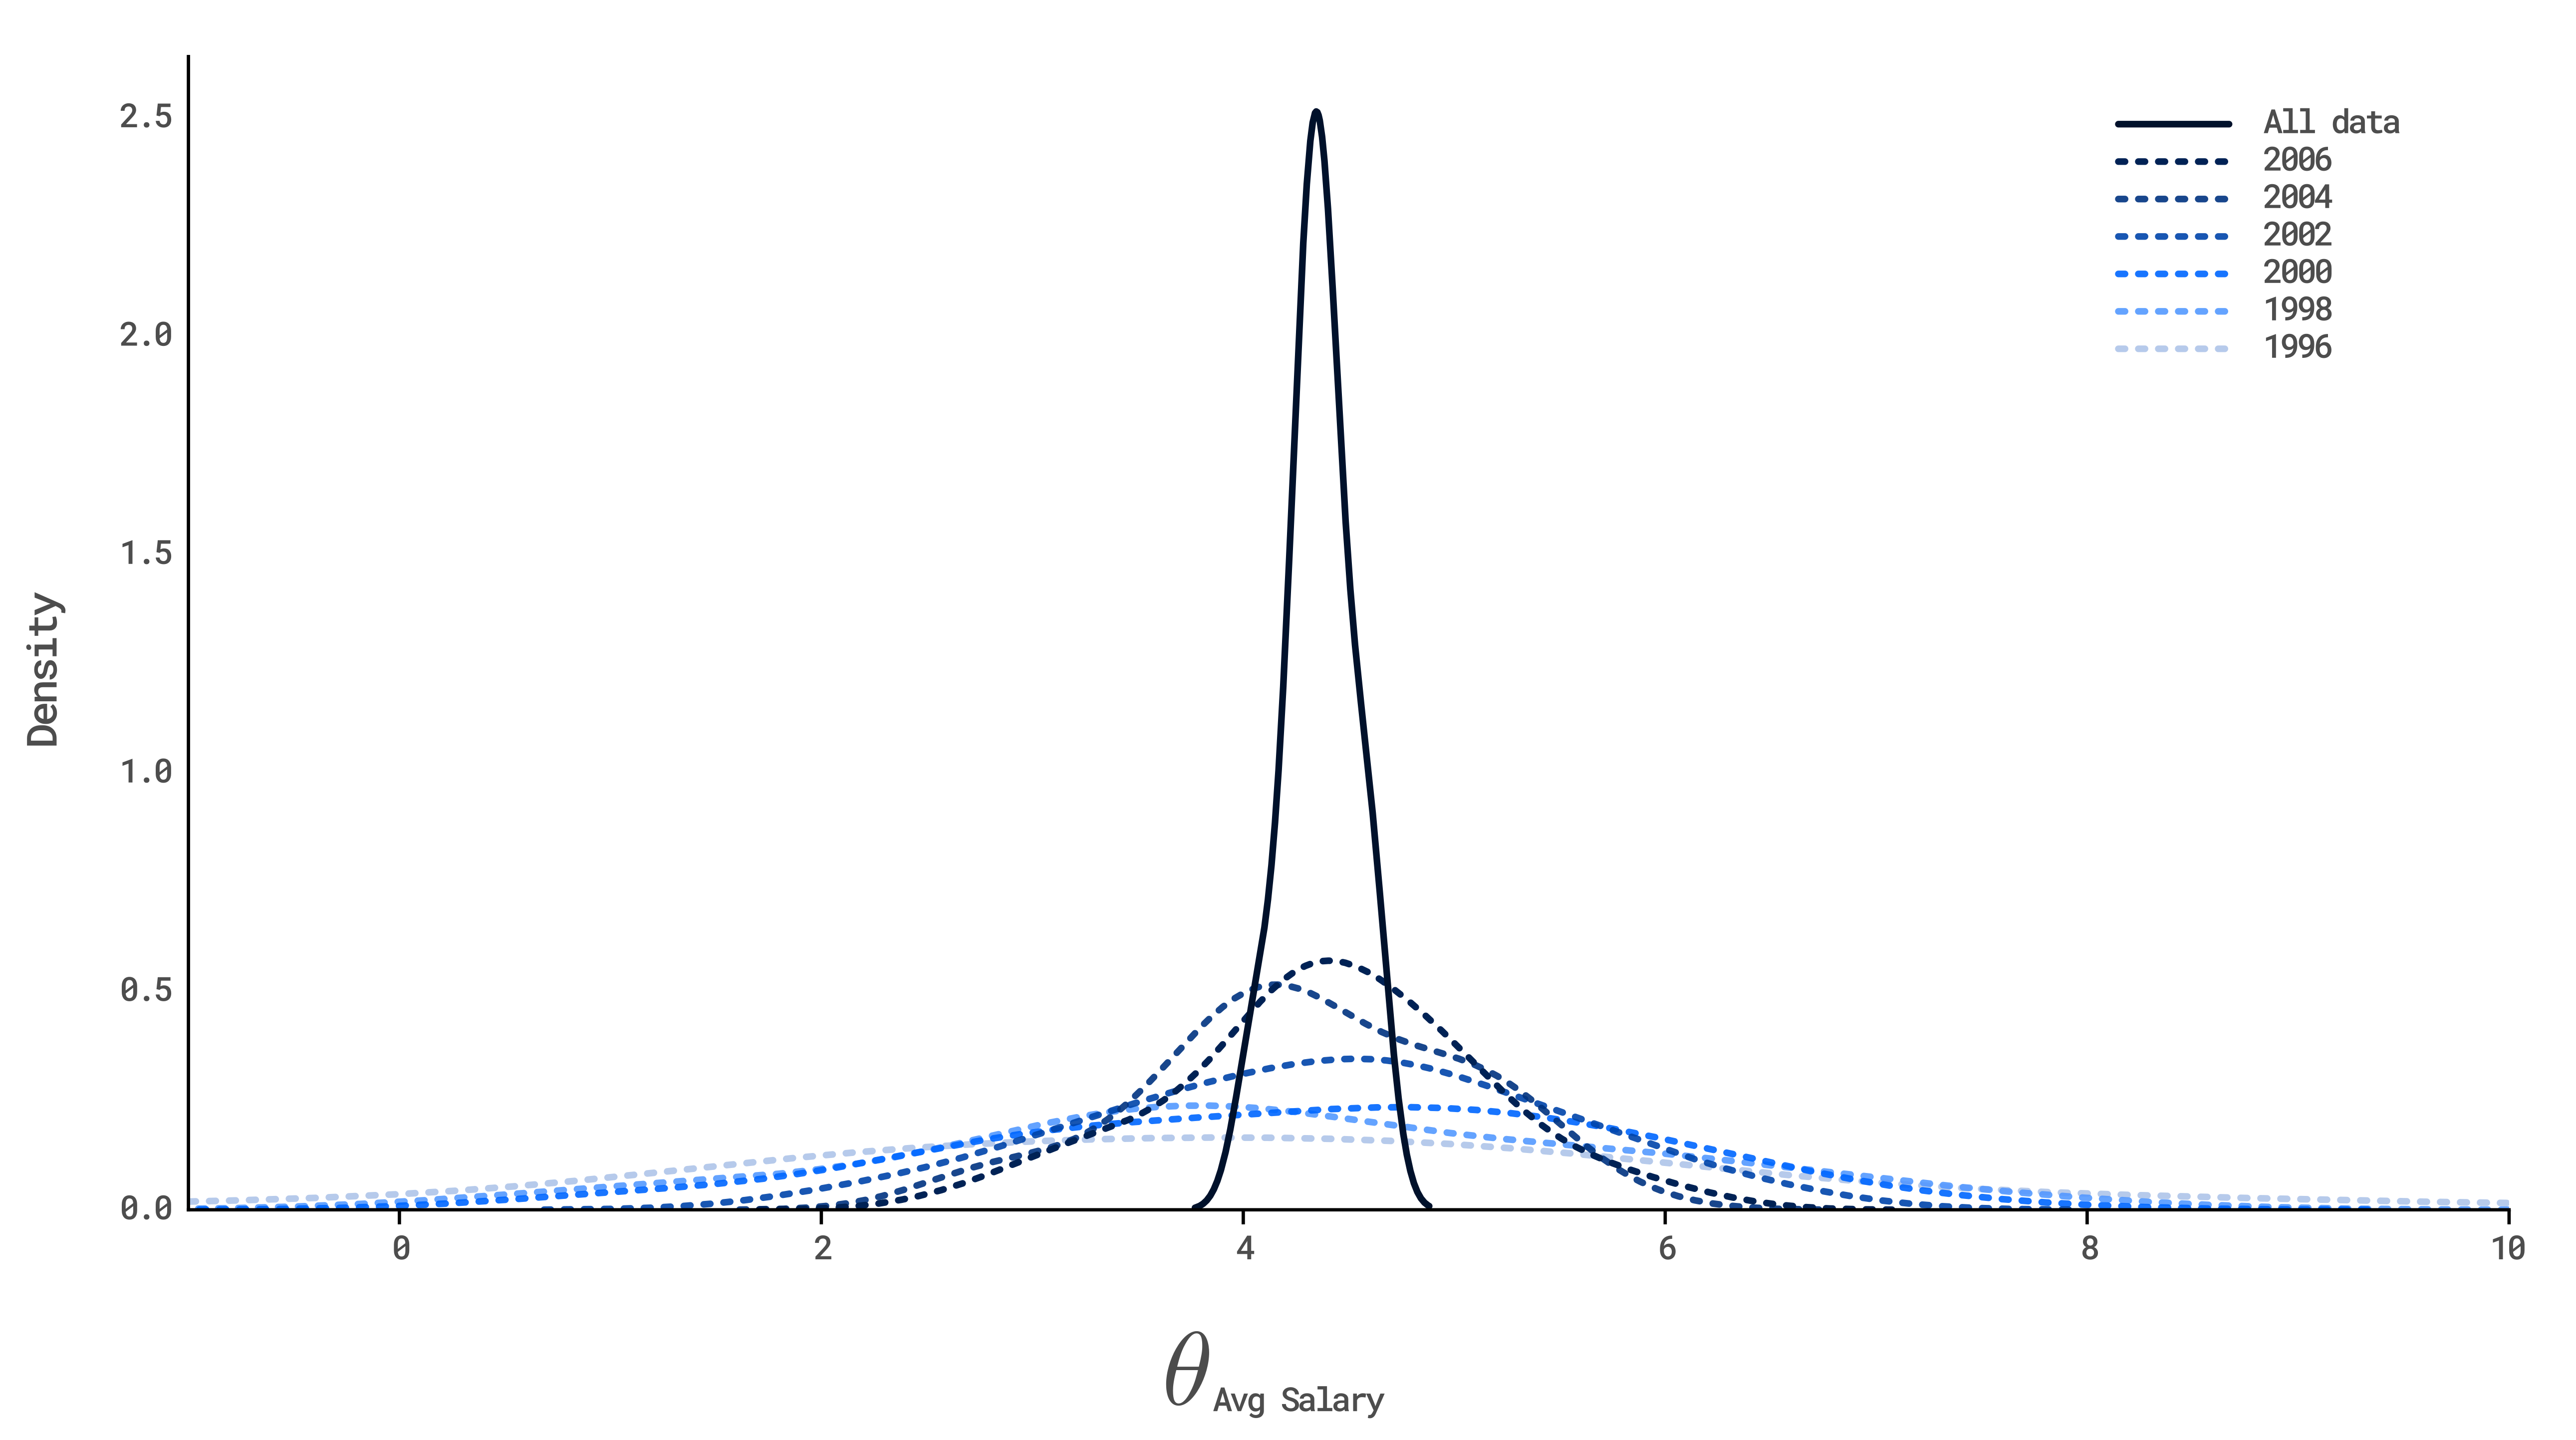
\includegraphics[width=0.75\textwidth]{images/ch5_online_learning/online_learning_salary.png}
    \setlength{\abovecaptionskip}{-10pt}
    \caption{Longitudinal analysis for model parameter - Avg. Salary (Intercept)}
    \label{fig:online_learning_salary}
\end{figure}

\begin{figure}[H]
    \centering
    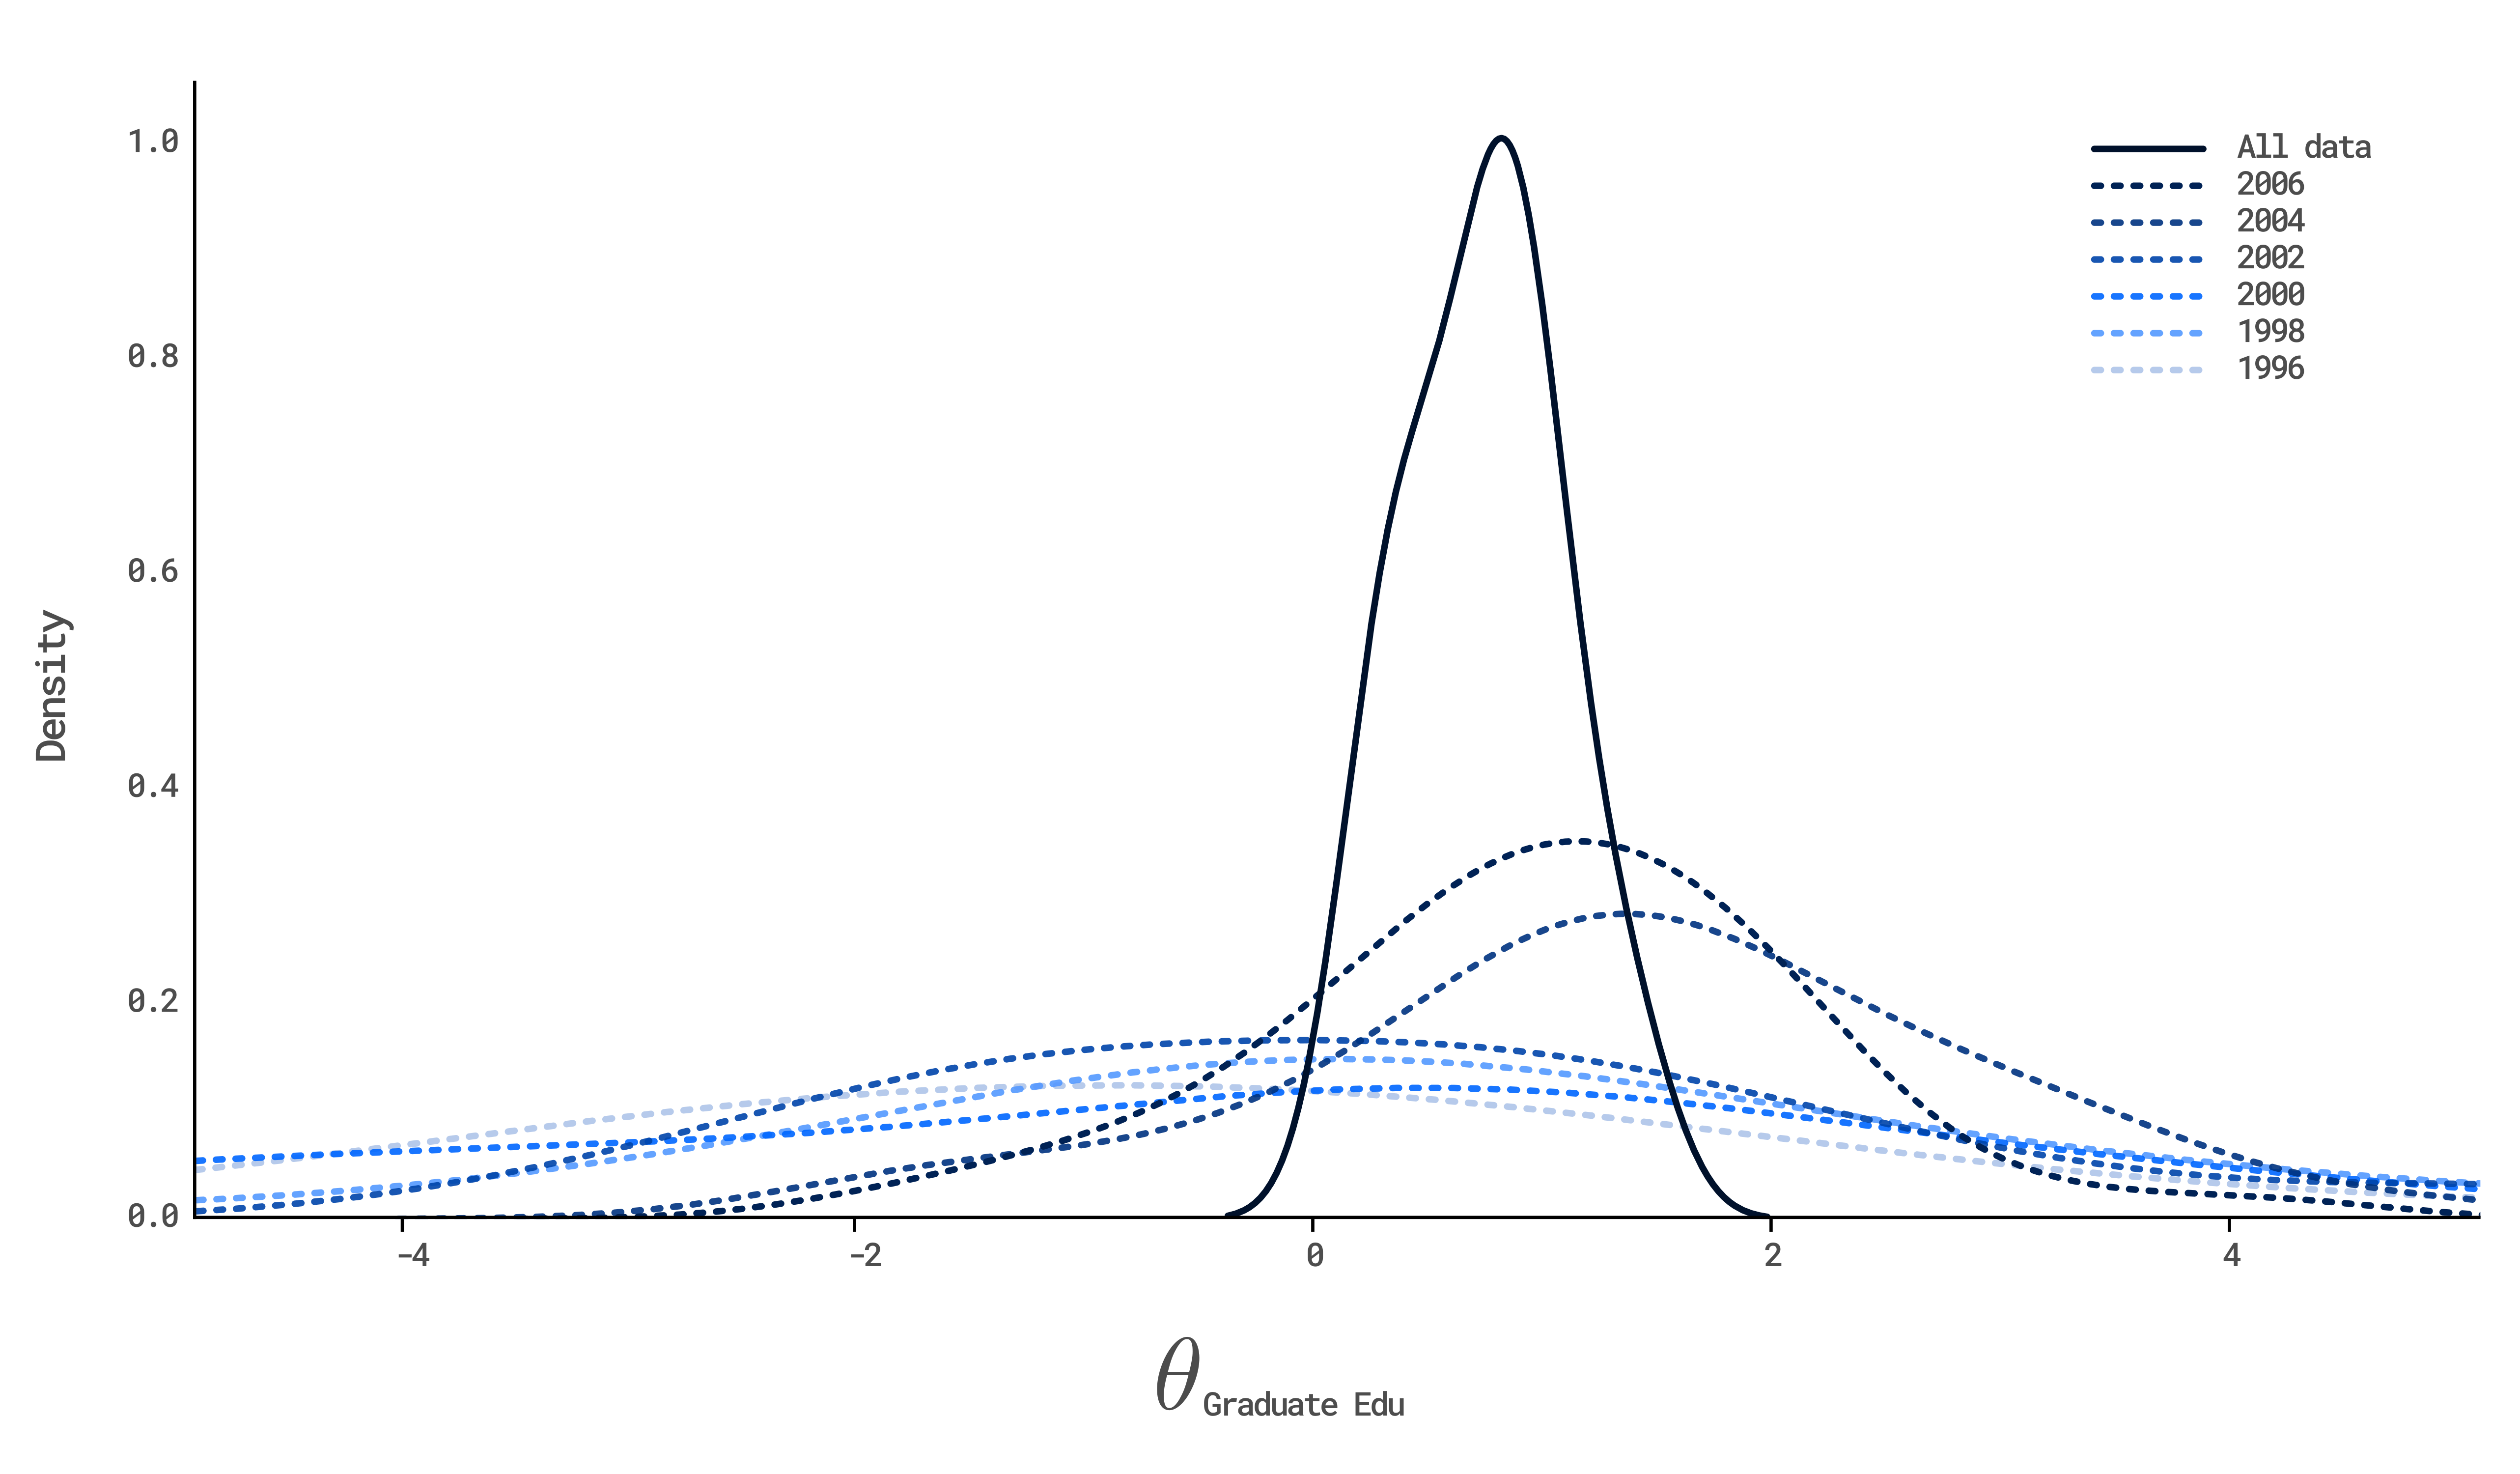
\includegraphics[width=0.8\textwidth]{images/ch5_online_learning/online_learning_grad.png}
    \caption{Longitudinal analysis for model parameter - Graduate Education Level }
    \label{fig:online_learning_grad}
\end{figure}

\begin{figure}[H]
    \centering
    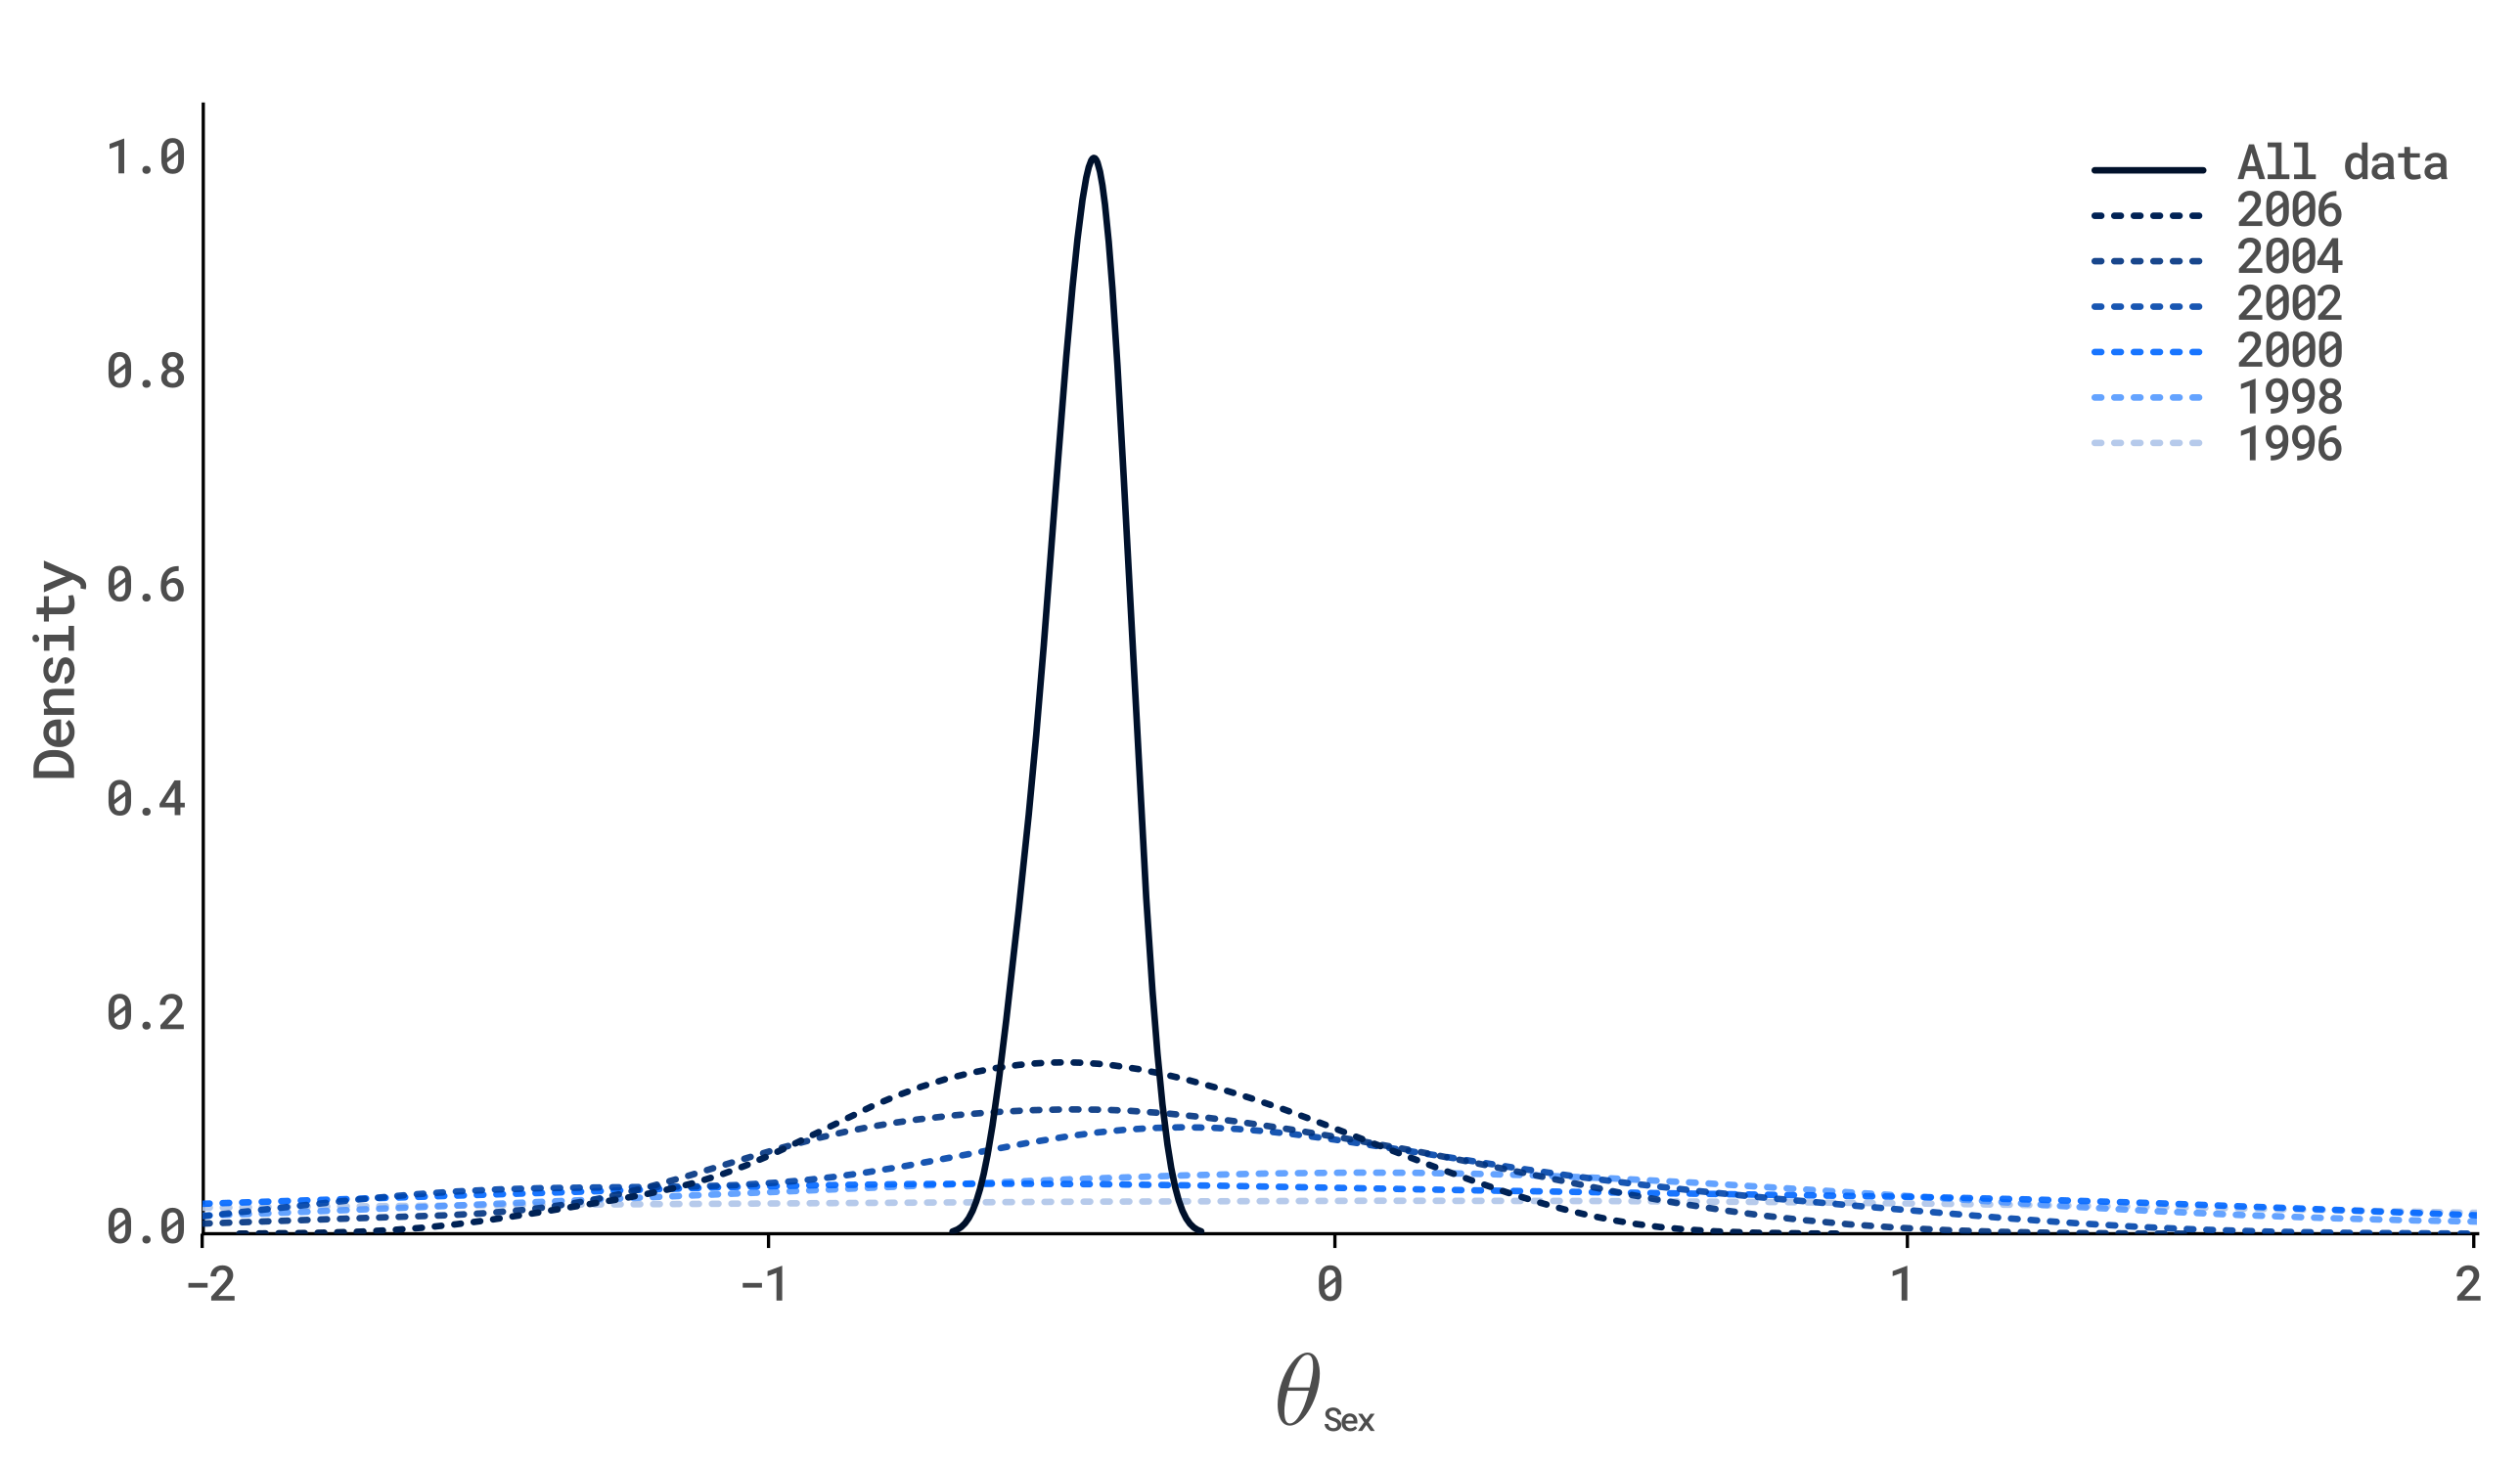
\includegraphics[width=0.8\textwidth]{images/ch5_online_learning/online_learning_gender.png}
    \caption{Longitudinal analysis for model parameter - Sex }
    \label{fig:online_learning_sex}
\end{figure}

The longitudinal analysis shows how the posterior distribution of each parameter is updated sequentially in light of new data. Starting from 1996, the priors are located at 0 for all model parameters, but the posteriors move towards the actual value each year. In the case of Average salary and Graduate level, they move positively, whereas in the case of Sex, they move negatively. As more data are available, the posterior distribution starts peaking around the true value, implying that the model is getting more confident in the parameter estimation. When comparing the posteriors using the whole dataset versus the sequential update (online learning), there is a difference in the density value. However, the peak of both scenarios is at the same point, which demonstrates that the Online learning setting produces reasonable estimates with a smaller dataset. 

Therefore, the Online Learning technique also allows an easy and natural way to update the model parameters because it resembles how data are generated. Also, the model is more robust to structural changes because it combines the past and current structure with the trend changes in the labour market. It requires less data and computational power because the estimation task is performed gradually. 
   
\section{Model validation}\label{section:model_validation}

While the in-sample metrics provide a general idea of how well the model fits the existing data, the out-of-sample performance measures the model's capability to generalize in the light of new data. That generalization determines whether the model captures the complex relationships between the model variables and ensures that the model does not “memorize” the noise in the data. Therefore, the out-of-sample evaluation assess the model's performance in a real setting. 

A graphical comparison between the true and the estimated salary distribution for the validation dataset is carried out to visually assess the potential use of the predicted distributions in a simulation setting, such as the labour market module in the ILUTE framework. This validation is performed in two levels: the aggregated that ensures the model is correctly representing salaries within different clusters observed in the data (e.g. salary distribution by industry, occupation, gender, and education level, among others) and the disaggregated that ensures the salary is being correctly predicted for each worker given their attributes.

\subsection{Aggregated level} 

The following charts show a comparison between the true salary distribution and the predicted salary distribution for different group variables, being industry and occupation, the most relevant groups given the hierarchical structure of the labour market. From these figures, it is observed that the model adequately represents the salary across all group variables regarding their shape and values.

\begin{figure}[H]
    \centering
    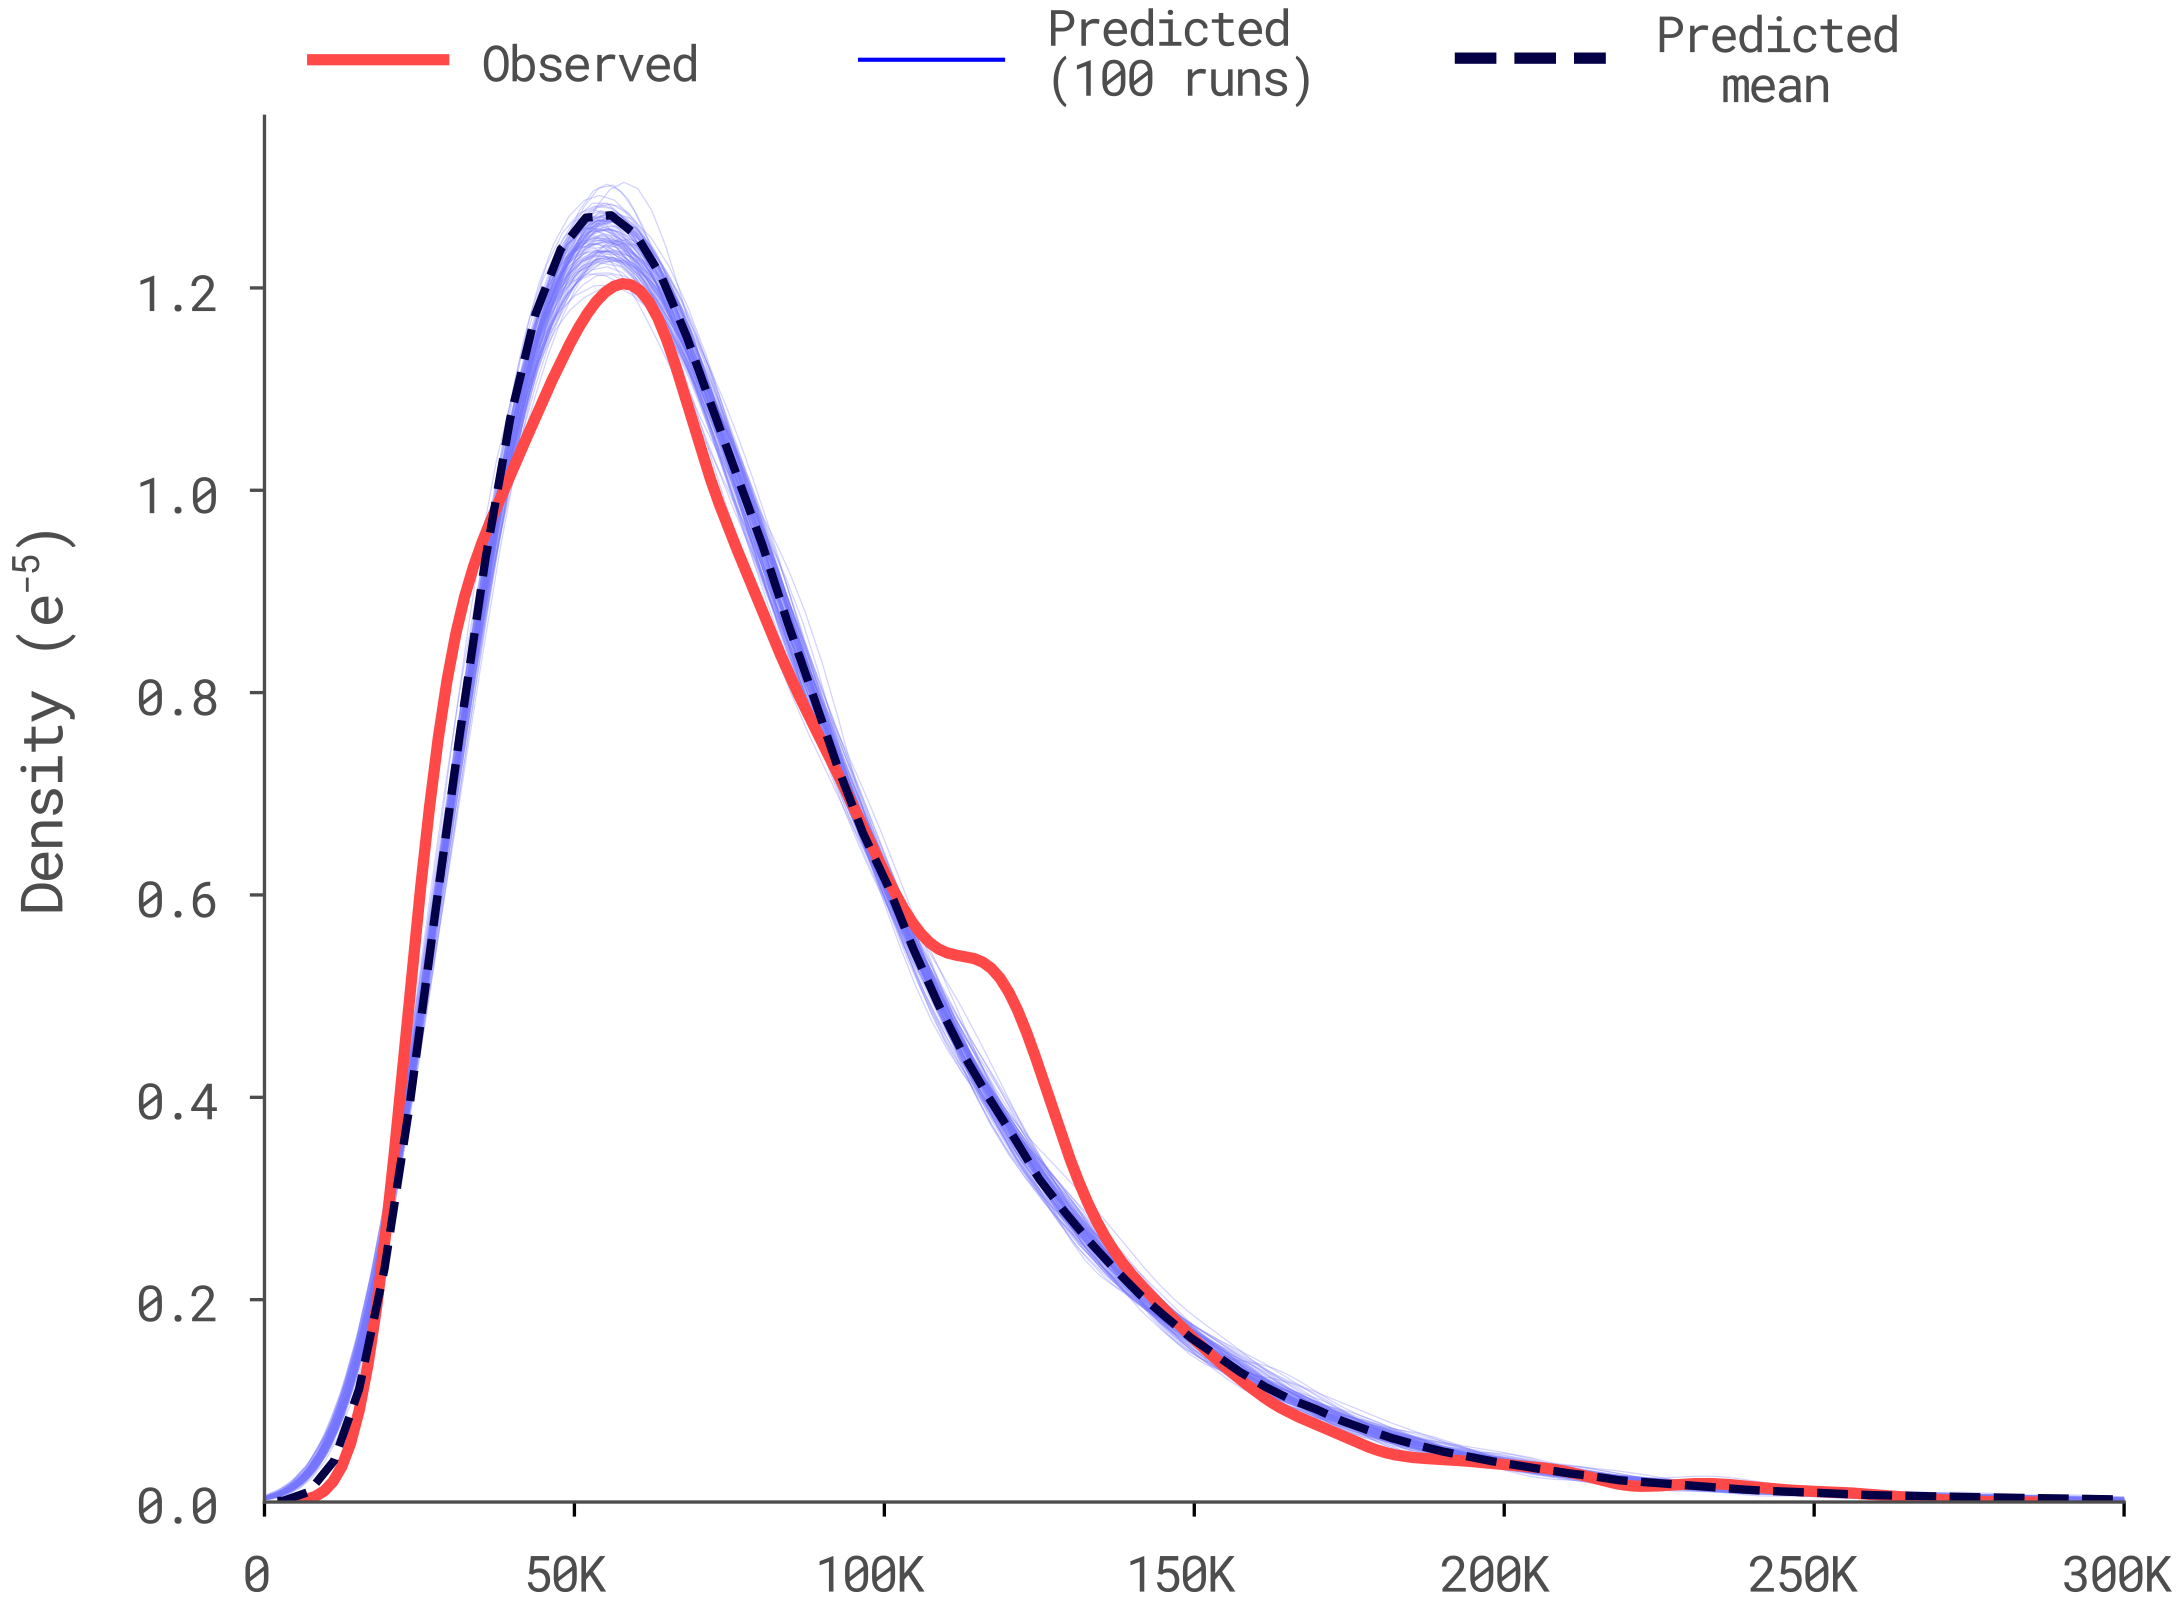
\includegraphics[width=0.7\textwidth]{images/ch5_agg_level/salary.png}
    \caption{Observed and predicted salary distribution for all individuals in the validation set}
    \setlength{\abovecaptionskip}{-10pt}
    \label{fig:validation_avg}
\end{figure}

\begin{landscape}
\begin{figure}[H]
    \centering
    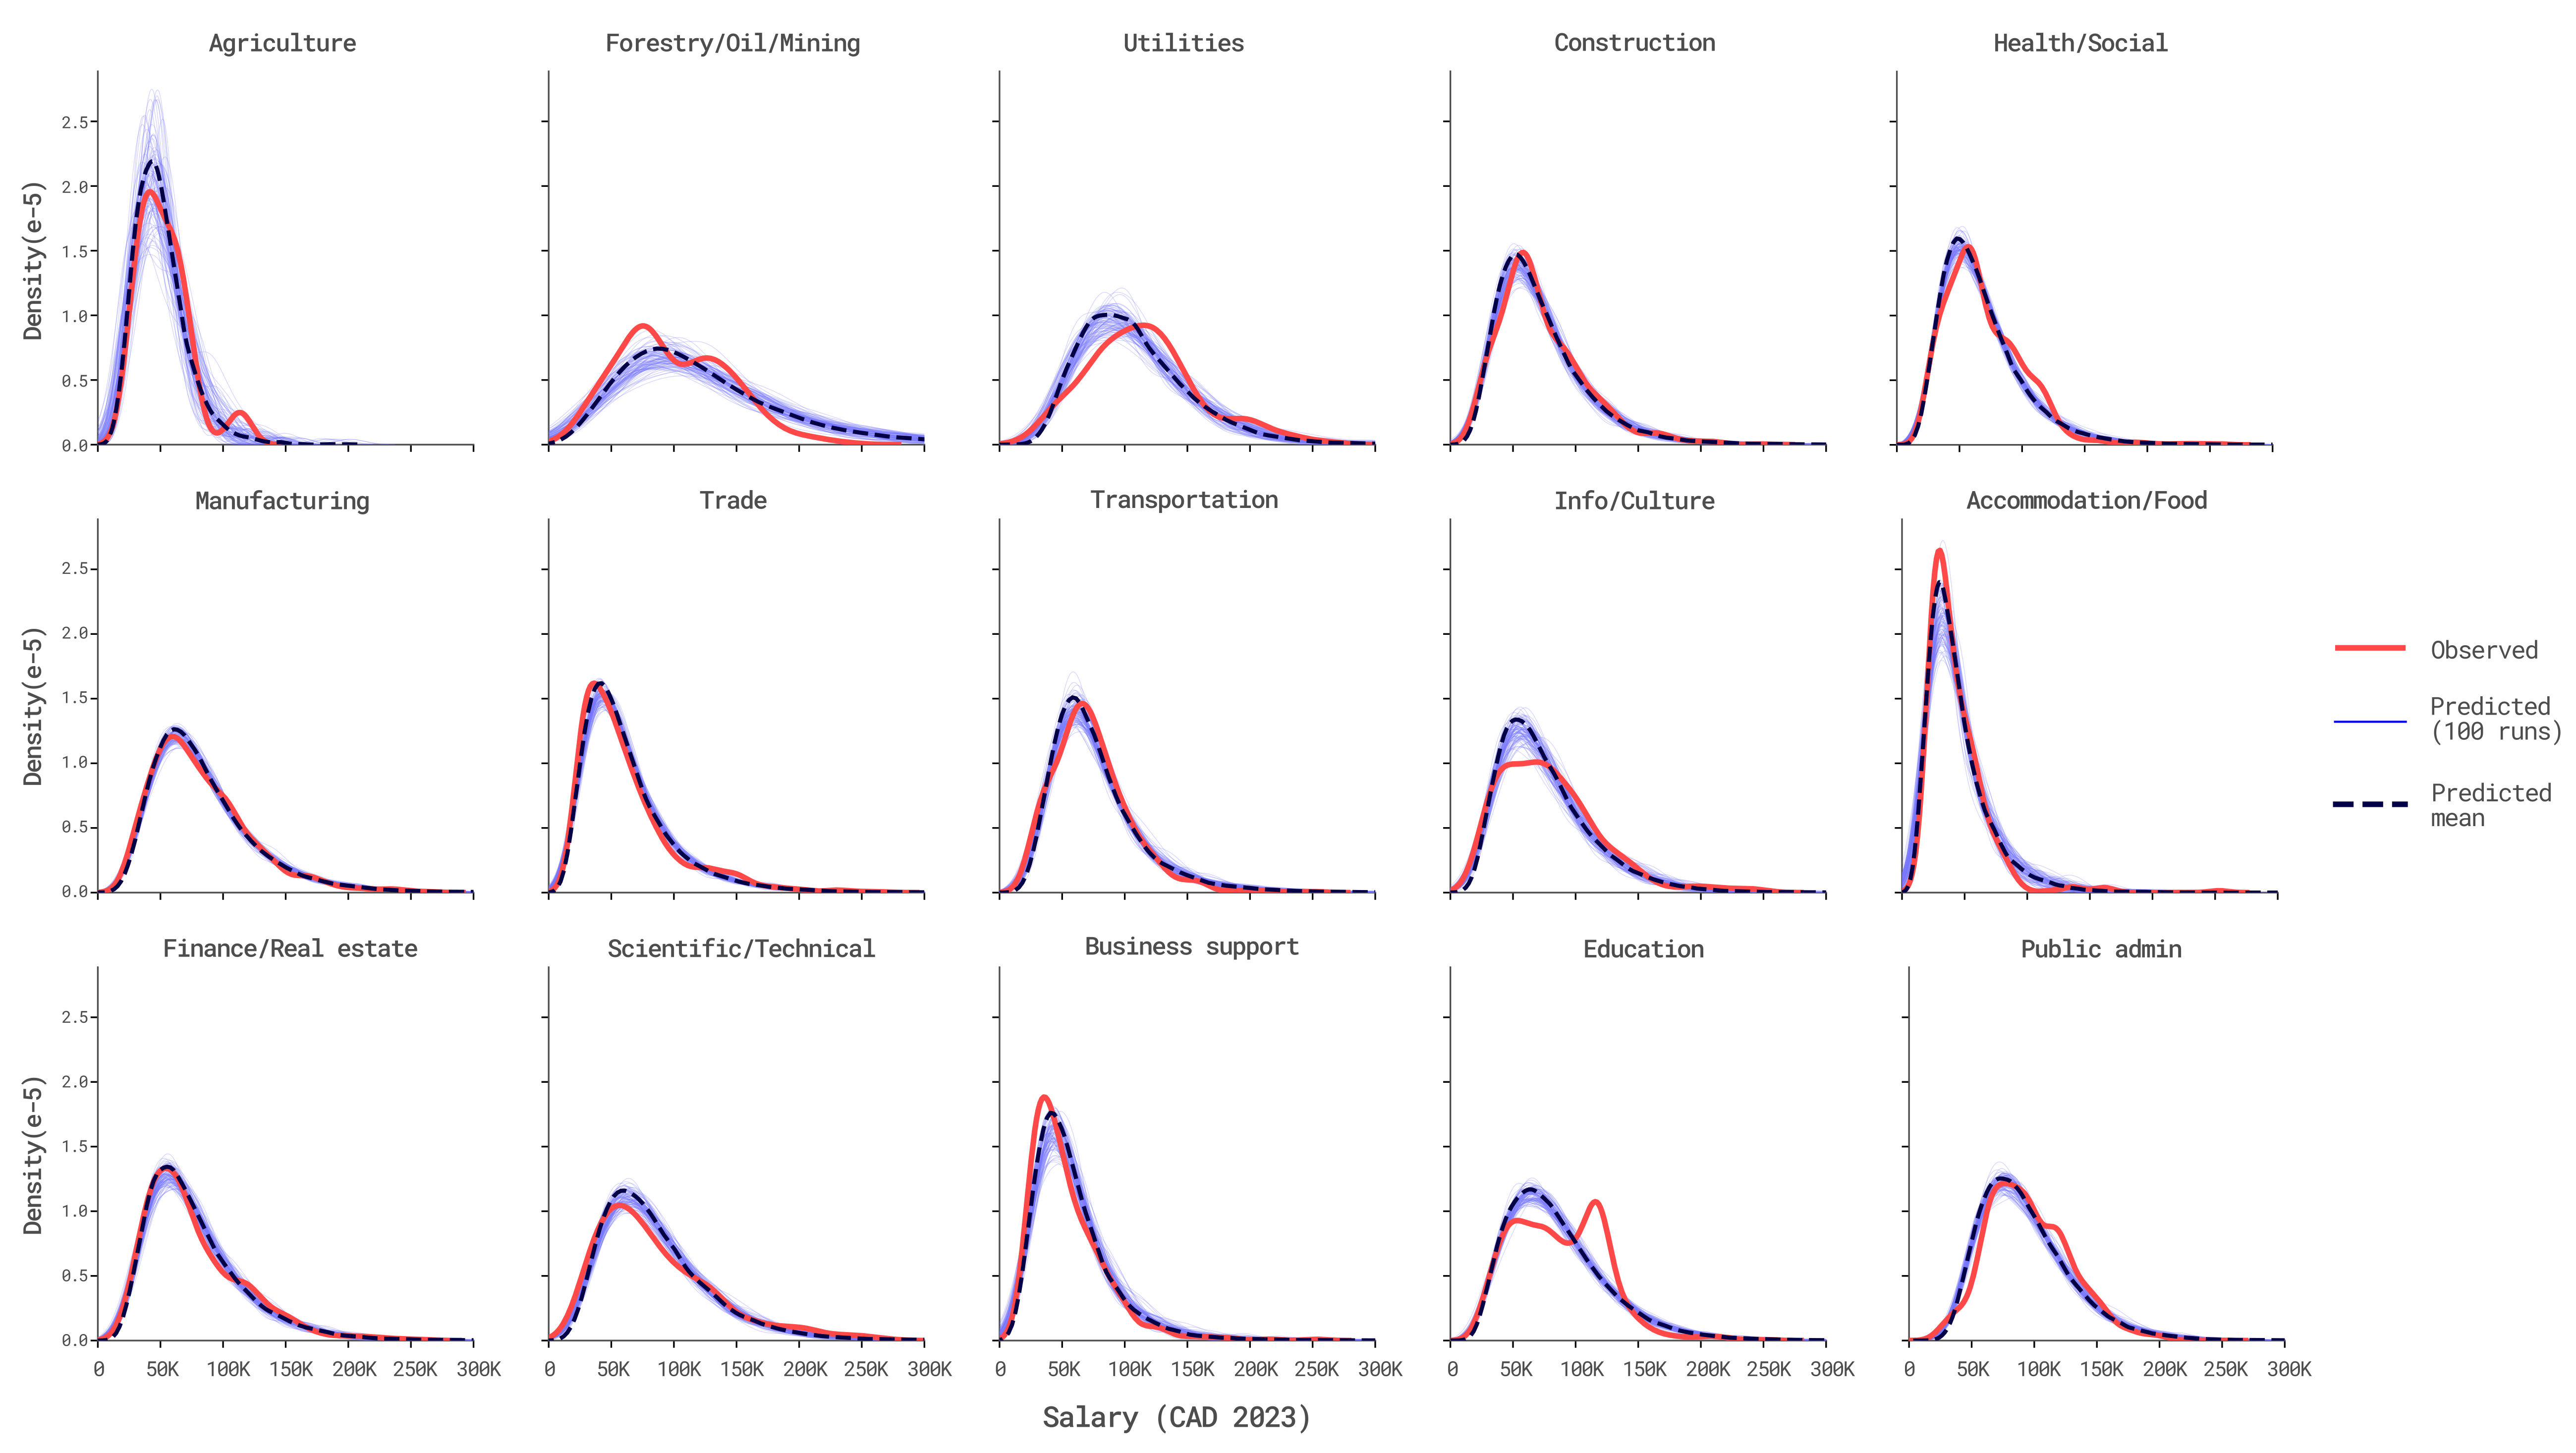
\includegraphics[width=1.3\textwidth]{images/ch5_agg_level/salary_ind.png}
    \caption{Observed and predicted salary distribution by Industry}
    \setlength{\abovecaptionskip}{-30pt}
    \label{fig:validation_industry}
\end{figure}


\begin{figure}[H]
    \centering
    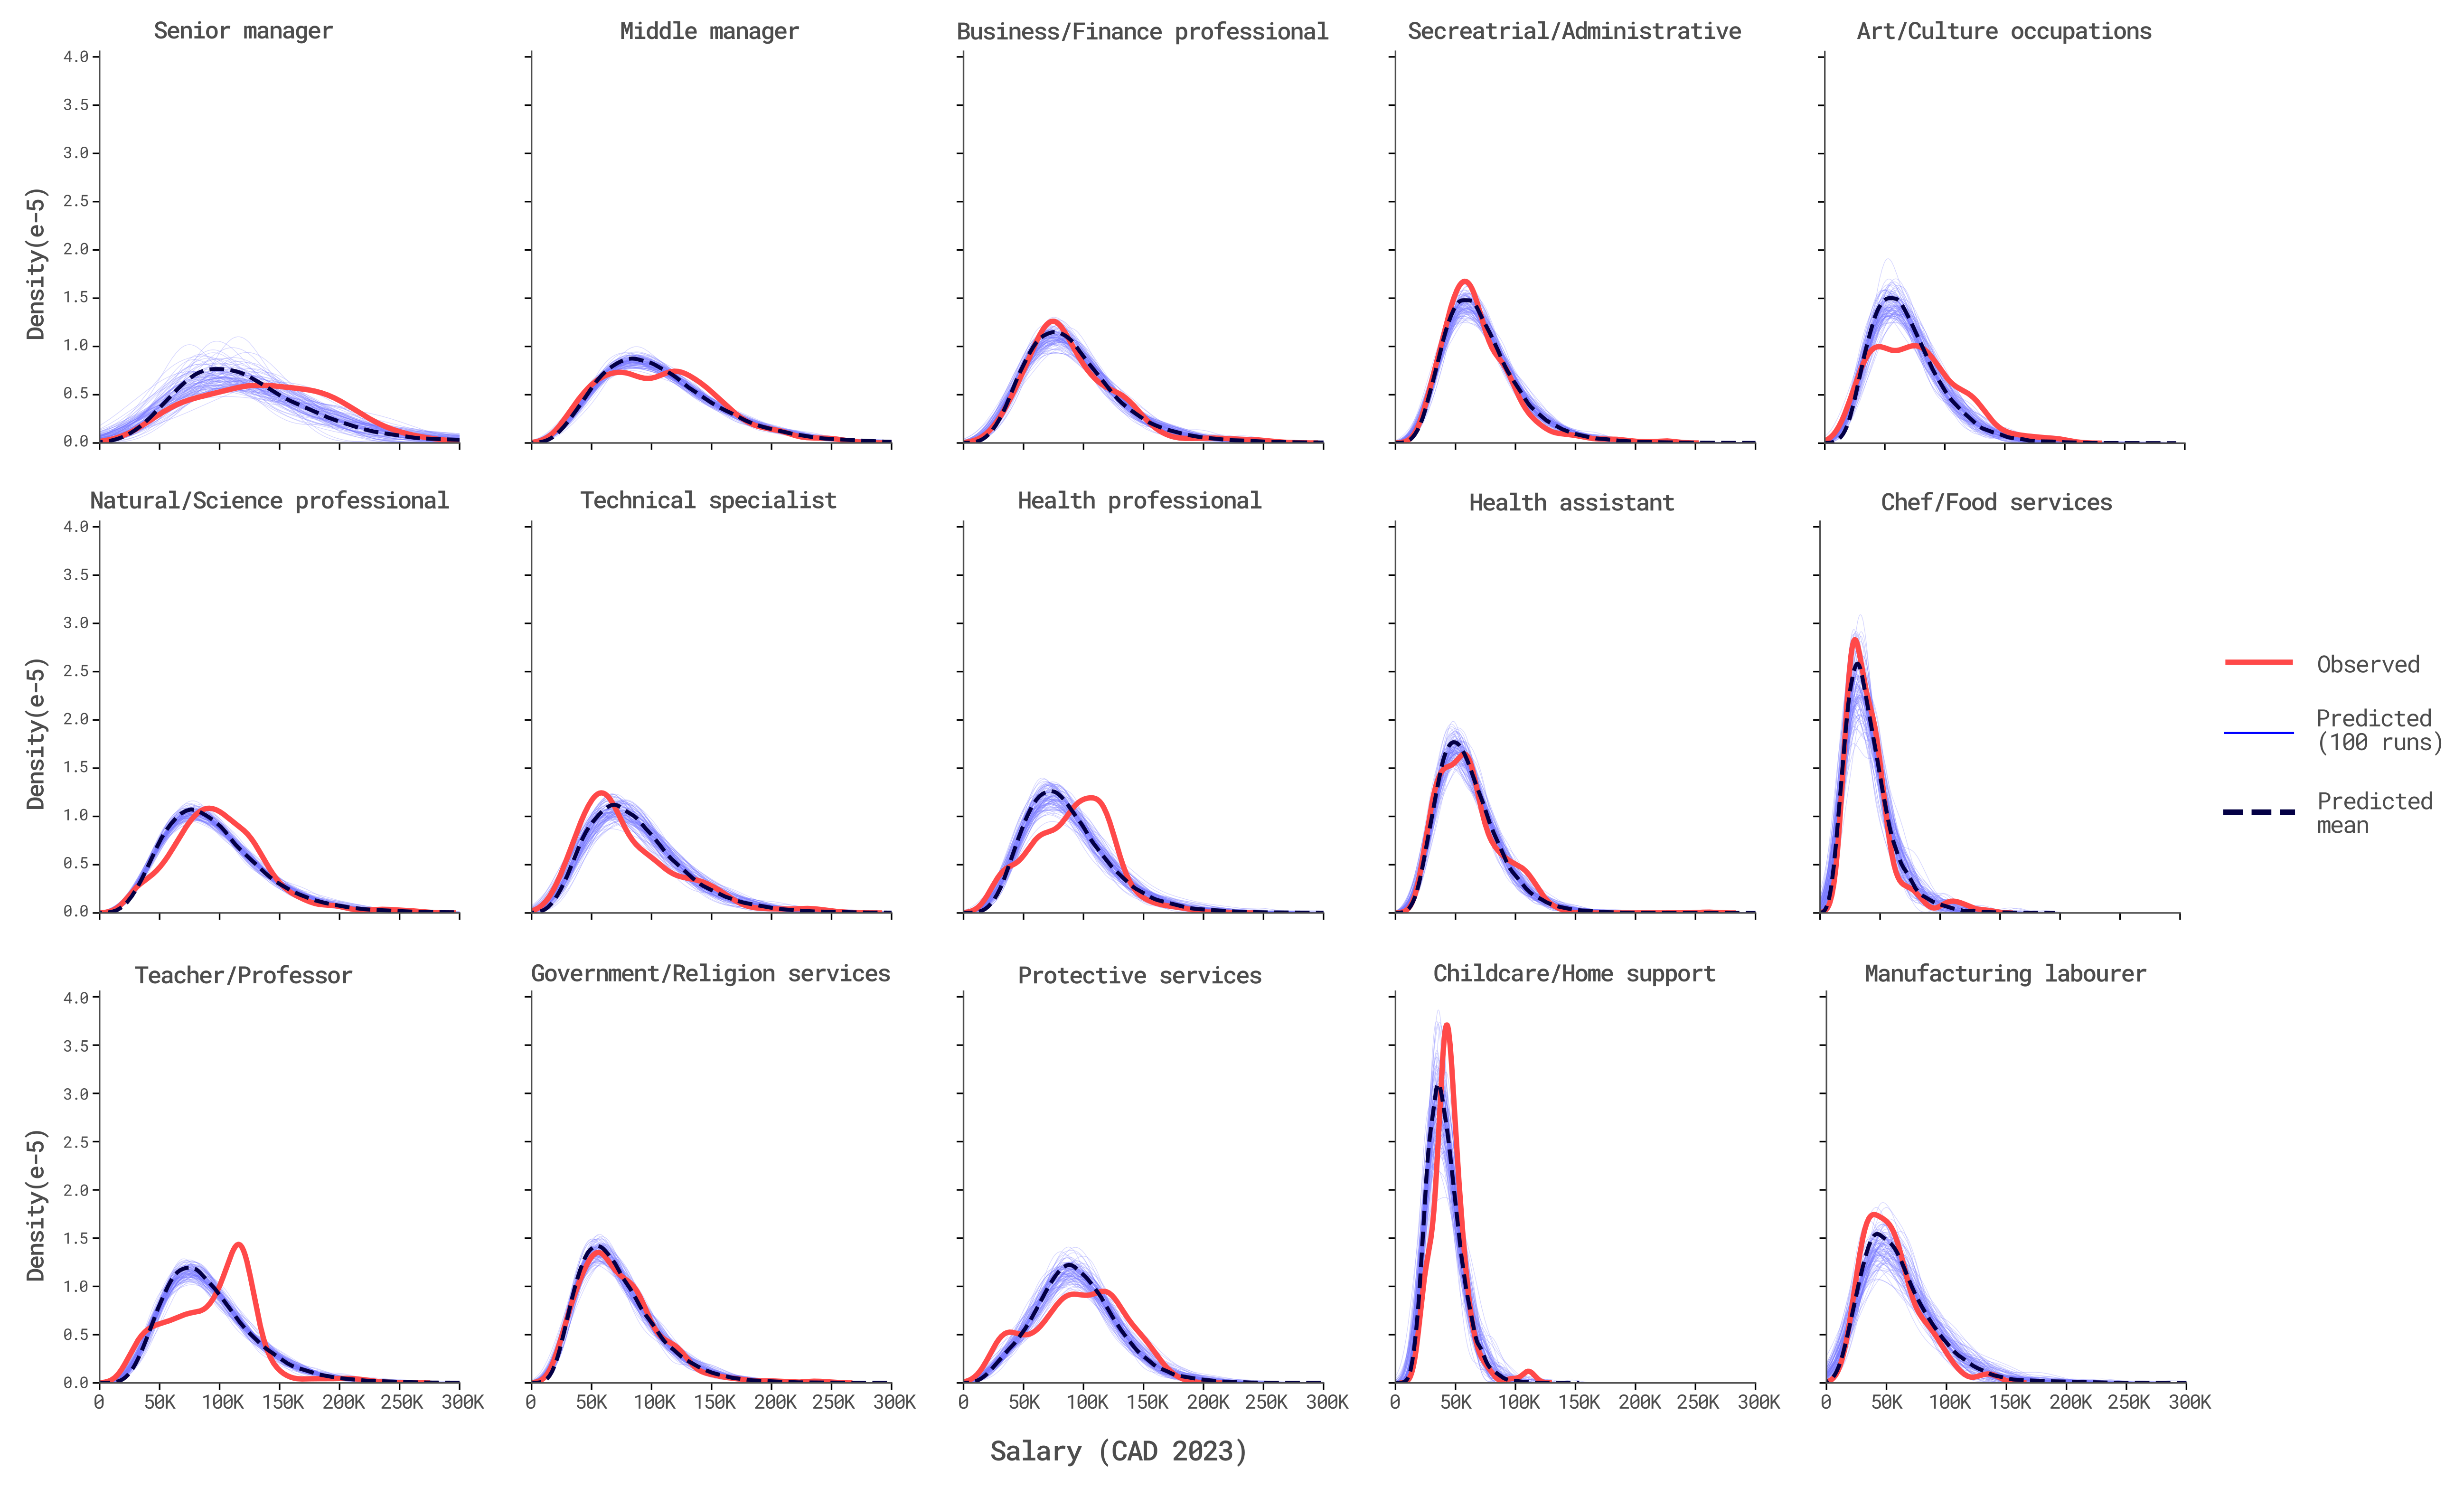
\includegraphics[width=1.3\textwidth]{images/ch5_agg_level/salary_occ.png}
    \caption{Observed and predicted salary distribution by Occupation}
    \setlength{\abovecaptionskip}{-15pt}
    \label{fig:validation_occupation}
\end{figure}
\end{landscape}

\subsection{Disaggregated level }

For the disaggregated level, \Cref{fig:validation_disagg} compares the following elements for a random set of workers. 

\begin{itemize}
    \item The observed salary: salary reported by the worker in the SLID. 

    \item The predicted salary: the expected value of the posterior salary distribution using the final model. 
    
    \item The posterior salary distribution is the estimated salary distribution for that worker given their attributes.
    
    \item The posterior salary distribution of similar workers: This is the reference case to compare with the previous distribution (posterior salary distribution) and represents the average salary distribution of workers with the same attributes (variables used in the model estimation). This distribution also allows us to identify whether the observed salary is an outlier compared to workers with the same characteristics. 
\end{itemize}

The comparison between these four elements provides a detailed perspective of the model's ability to represent data at the disaggregated level. The comparison between the observed salary and the posterior salary distribution of similar workers illustrates the stochastic nature of salaries. Given the size of the validation dataset, it is unfeasible to report this chart for all workers. However, the GitHub repository of this thesis provides a Jupyter notebook that allows to explore and create this chart for any worker in the dataset. 

\begin{landscape}
    \begin{figure}[H]
        \centering
        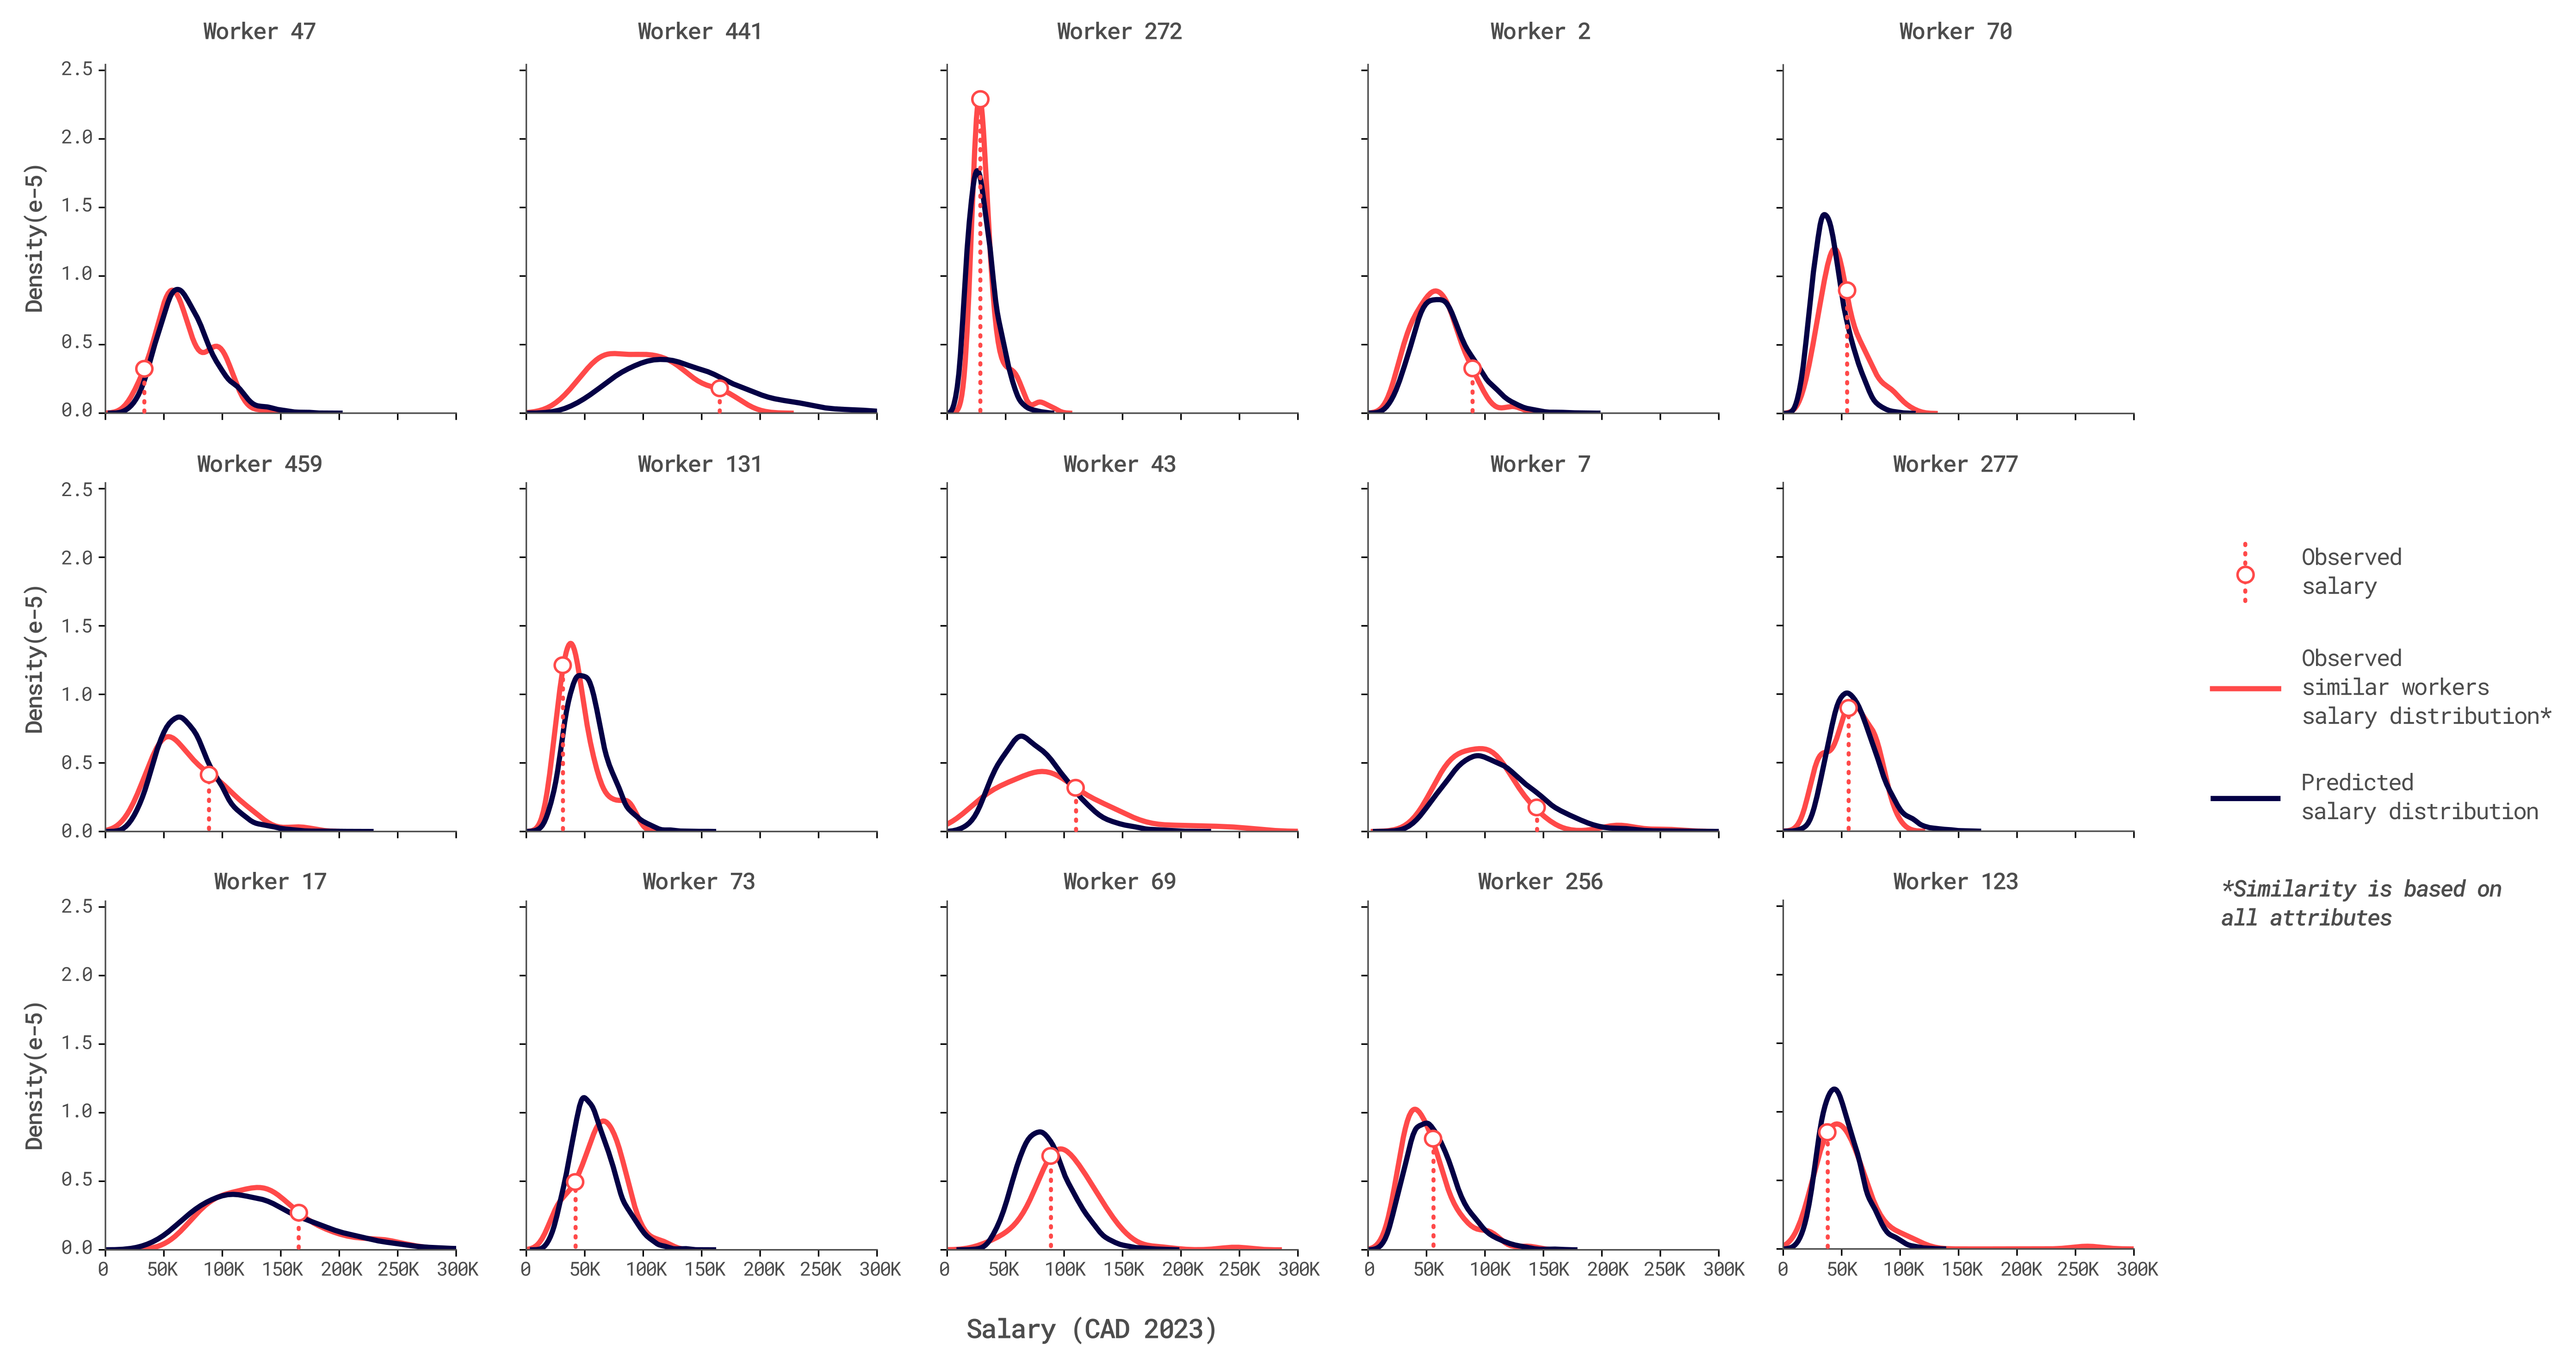
\includegraphics[width=1.3\textwidth]{images/ch5_disagg_level/workers.png}
        \caption{Disaggregated analysis of salary distribution for 15 random selected workers within the validation dataset}
        \setlength{\abovecaptionskip}{-10pt}
        \label{fig:validation_disagg}
    \end{figure}
\end{landscape}



